% main.tex — standalone wrapper that compiles Chapter 4 to a PDF.
% To integrate into a larger thesis: drop % chapter4.tex — Software Design and Implementation.
% Verified against locked-demo head: tag baremetal-mnist-fc-demo-locked.

% Restart counters so this chapter is self-contained.
\setcounter{section}{0}
\setcounter{figure}{0}
\setcounter{table}{0}
\setcounter{lstlisting}{0}

% =====================================================================
\section{Design Requirements}
\label{sec:ch4-req}
% =====================================================================

The software stack supporting the CGRA-accelerated MNIST inference demo
must satisfy three orthogonal classes of requirements: \textbf{data-path
correctness}, \textbf{control-path determinism}, and \textbf{subsystem
coordination}. The data path orchestrates the migration of 28$\times$28
input images, 105~KB of pre-quantized weight blobs, and per-layer
activations between three storage tiers --- DDR3 main memory
(\addr{00200000}--\addr{002FFFFF}), the CGRA tile memory
(4 banks $\times$ 4~KiB SRAM, accessed through the
\addr{10000000} window), and the per-PE scratchpad
(1024 words $\times$ 32 bits per Processing Element, accessed through the
\addr{40000000} window). The software must marshal each layer's input
tensor into the correct memory region, configure the integrated DMA
controller with the appropriate source/destination/length triple, and
recover the layer's output activations through a memory-mapped result
register file without violating the AXI4 burst contract or the CGRA
accumulator's 40-bit saturation envelope.

\begin{sloppypar}
The control path must, simultaneously, configure the CGRA's 16 Processing
Elements (PEs) into a context-multiplexed dense-matrix-multiply kernel
and trigger the Control Unit (CU) to execute that kernel deterministically
--- without operating-system jitter, cache-line interference, or interrupt
latency that would corrupt the cycle-counter measurements forming the
thesis' performance claims. To meet this constraint, the implementation
is hosted on a bare-metal Cortex-A9 ELF rather than under Linux: the host
code runs from on-chip memory (OCM), drives the CGRA through its
30-register APB control-status register (CSR) file, and renders results
to an HDMI framebuffer in DDR through a direct memory-mapped IO pattern,
with no operating system in the critical loop. This design preserves a
sub-1\% jitter envelope on the per-frame cycle measurements while still
supporting a real-time visual demonstration to a defense audience.
\end{sloppypar}

% =====================================================================
\section{Software Design}
\label{sec:ch4-design}
% =====================================================================

\subsection{System Software Architecture}
\label{ssec:arch}

Before describing the per-frame execution flow, this subsection
establishes the high-level layering of the software stack and the
hardware blocks it drives. Figure~\ref{fig:arch} gives a block-diagram
view of the complete system: the application code on the left talks
to the CGRA accelerator on the right through two distinct interfaces
--- a narrow control plane over APB and a wide data plane over AXI4 ---
and both sides share a single DDR3 memory through which all bulk
operands pass.

\begin{figure}[!htbp]
\centering
\resizebox{\textwidth}{!}{%
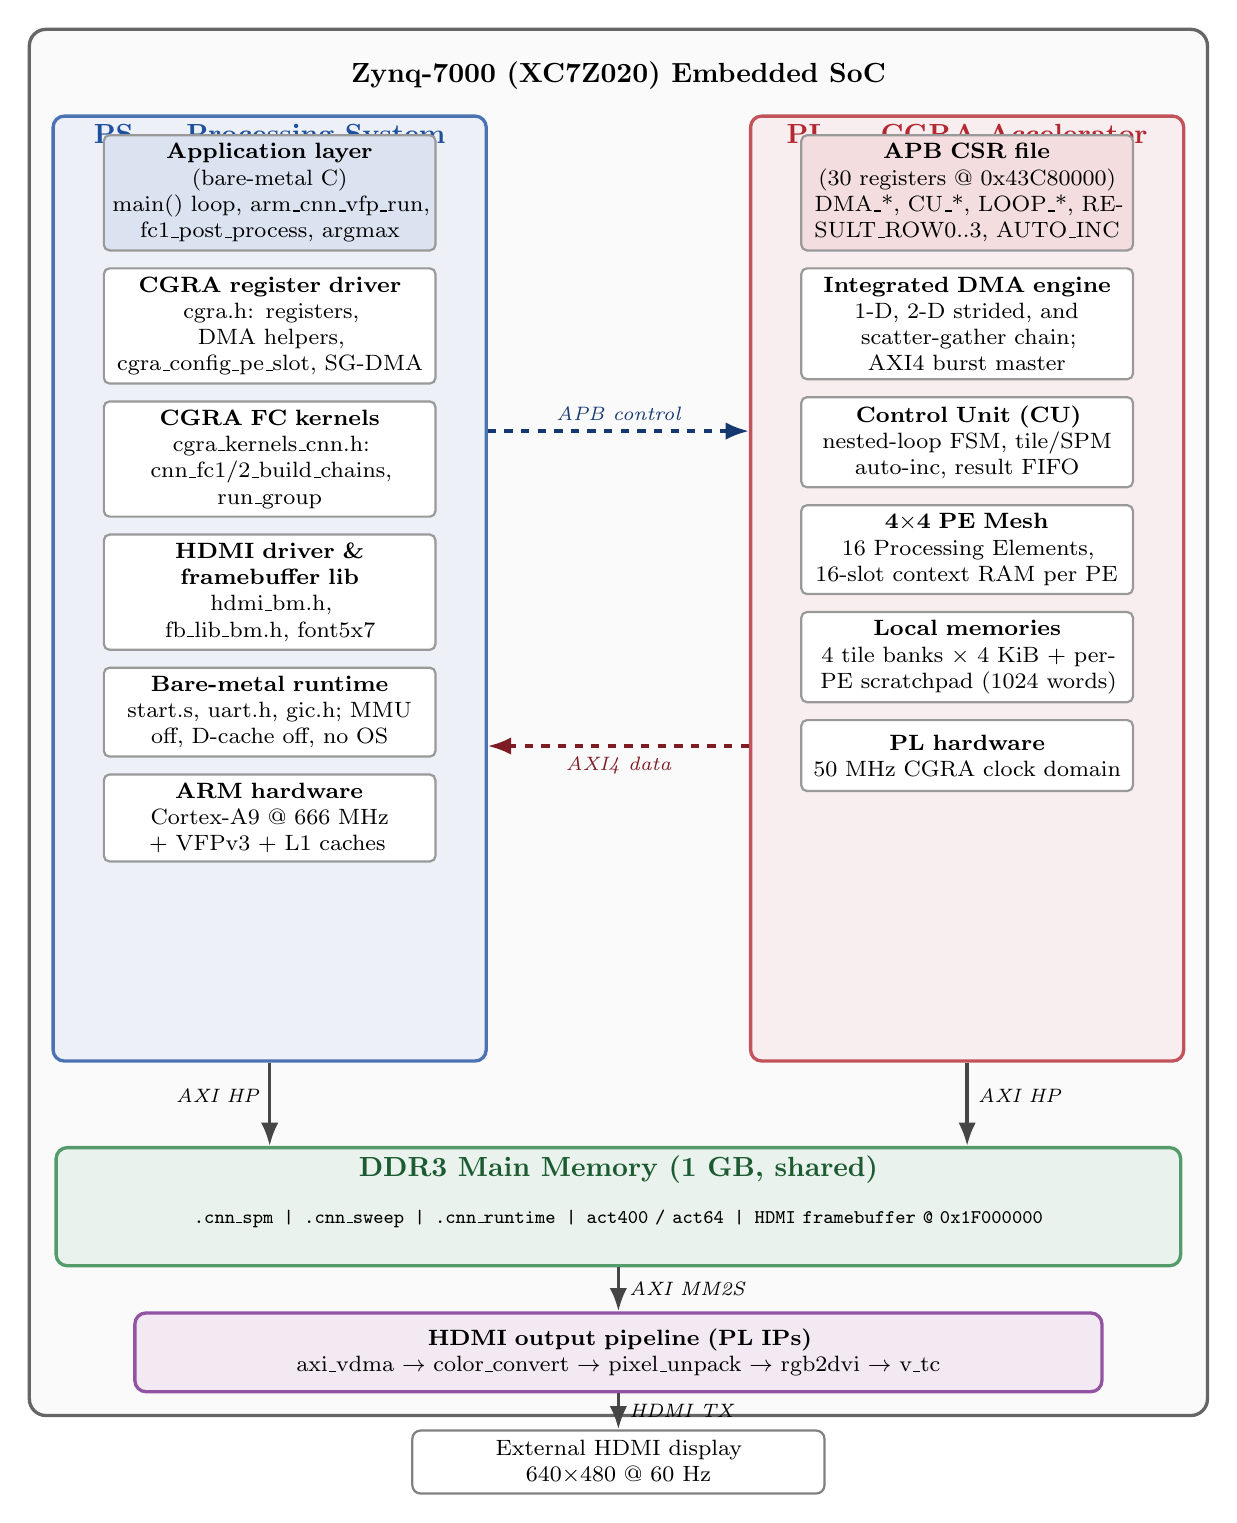
\begin{tikzpicture}[
    node distance = 2.5cm and 3cm,
    every node/.append style = {font=\footnotesize},
    soc/.style    = {rectangle, draw=black!60, fill=gray!4, very thick,
                     rounded corners=6pt, inner sep=8pt},
    psbox/.style  = {rectangle, draw=armblue!80, fill=armblue!8,
                     very thick, rounded corners=4pt, align=center,
                     minimum width=5.5cm, minimum height=12cm,
                     inner sep=4pt},
    plbox/.style  = {rectangle, draw=cgrared!80, fill=cgrared!8,
                     very thick, rounded corners=4pt, align=center,
                     minimum width=5.5cm, minimum height=12cm,
                     inner sep=4pt},
    ddrbox/.style = {rectangle, draw=ddrgreen!80, fill=ddrgreen!10,
                     very thick, rounded corners=4pt, align=center,
                     text width=14cm, minimum height=1.5cm,
                     inner sep=4pt},
    hdmibx/.style = {rectangle, draw=hdmipurple!80, fill=hdmipurple!10,
                     very thick, rounded corners=4pt, align=center,
                     text width=12cm, minimum height=1cm,
                     inner sep=4pt},
    extbx/.style  = {rectangle, draw=black!50, fill=white, thick,
                     rounded corners=3pt, align=center,
                     text width=5cm, minimum height=0.8cm},
    %% KEY FIX (user request 2): every inner block has text width=4cm so
    %% long sentences wrap into multiple lines instead of pushing the
    %% block width outward and colliding with the neighbouring lane.
    inner/.style  = {rectangle, draw=black!40, fill=white, thick,
                     rounded corners=2pt, align=center,
                     text width=4cm, inner sep=3pt,
                     minimum height=0.9cm, font=\footnotesize},
    blocktitle/.style = {font=\bfseries, anchor=north},
    busArr/.style = {-Latex, very thick, draw=gray!55!black},
    apbArr/.style = {-Latex, very thick, draw=armblue!70!black, dashed},
    dmaArr/.style = {-Latex, very thick, draw=cgrared!70!black, dashed},
    labelArr/.style = {font=\scriptsize\itshape}
]

% ===== Title bar =====
\node[font=\bfseries] (title) at (0, 7.2)
   {Zynq-7000 (XC7Z020) Embedded SoC};

% ===== PS side (left) =====
\node[psbox, anchor=north west] (ps) at (-7.2, 6.7) {};
\node[blocktitle] at (ps.north)
   {\textcolor{armblue}{PS --- Processing System}};

\node[inner, fill=armblue!16, below=2.5mm of ps.north] (app)
   {\textbf{Application layer} \\ (bare-metal C) \\
    main() loop, arm\_cnn\_vfp\_run, fc1\_post\_process, argmax};
\node[inner, below=2mm of app] (drvA)
   {\textbf{CGRA register driver} \\
    cgra.h: registers, DMA helpers, cgra\_config\_pe\_slot, SG-DMA};
\node[inner, below=2mm of drvA] (drvB)
   {\textbf{CGRA FC kernels} \\
    cgra\_kernels\_cnn.h: cnn\_fc1/2\_build\_chains, run\_group};
\node[inner, below=2mm of drvB] (drvC)
   {\textbf{HDMI driver \& framebuffer lib} \\
    hdmi\_bm.h, fb\_lib\_bm.h, font5x7};
\node[inner, below=2mm of drvC] (rt)
   {\textbf{Bare-metal runtime} \\
    start.s, uart.h, gic.h; MMU off, D-cache off, no OS};
\node[inner, below=2mm of rt] (hw)
   {\textbf{ARM hardware} \\
    Cortex-A9 @ 666 MHz + VFPv3 + L1 caches};

% ===== PL side (right) =====
\node[plbox, anchor=north east] (pl) at (7.2, 6.7) {};
\node[blocktitle] at (pl.north)
   {\textcolor{cgrared}{PL --- CGRA Accelerator}};

\node[inner, fill=cgrared!16, below=2.5mm of pl.north] (csr)
   {\textbf{APB CSR file} \\ (30 registers @ 0x43C80000) \\
    DMA\_*, CU\_*, LOOP\_*, RESULT\_ROW0..3, AUTO\_INC};
\node[inner, below=2mm of csr] (dma)
   {\textbf{Integrated DMA engine} \\
    1-D, 2-D strided, and scatter-gather chain; AXI4 burst master};
\node[inner, below=2mm of dma] (cu)
   {\textbf{Control Unit (CU)} \\
    nested-loop FSM, tile/SPM auto-inc, result FIFO};
\node[inner, below=2mm of cu] (mesh)
   {\textbf{4$\times$4 PE Mesh} \\
    16 Processing Elements, 16-slot context RAM per PE};
\node[inner, below=2mm of mesh] (mem)
   {\textbf{Local memories} \\
    4 tile banks $\times$ 4 KiB + per-PE scratchpad (1024 words)};
\node[inner, below=2mm of mem] (clk)
   {\textbf{PL hardware} \\
    50 MHz CGRA clock domain};

% ===== Bus arrows between PS and PL =====
\coordinate (ap1) at ($(ps.east)+(0,2.0)$);
\coordinate (ap2) at ($(pl.west)+(0,2.0)$);
\coordinate (dm1) at ($(pl.west)+(0,-2.0)$);
\coordinate (dm2) at ($(ps.east)+(0,-2.0)$);

\draw[apbArr] (ap1) -- (ap2)
   node[midway, above, labelArr, text=armblue!70!black]{APB control};
\draw[dmaArr] (dm1) -- (dm2)
   node[midway, below, labelArr, text=cgrared!70!black]{AXI4 data};

% ===== DDR =====
\node[ddrbox, anchor=north] (ddr) at (0, -6.4) {};
\node[blocktitle, anchor=north] at (ddr.north)
   {\textcolor{ddrgreen!70!black}{DDR3 Main Memory (1 GB, shared)}};
\node[anchor=center, font=\scriptsize\ttfamily, align=center,
      text width=13cm] at ($(ddr.center)+(0,-0.15)$) {
   .cnn\_spm \,|\, .cnn\_sweep \,|\, .cnn\_runtime \,|\,
   act400 / act64 \,|\, HDMI framebuffer @ 0x1F000000
};

% Vertical buses PS <-> DDR and PL <-> DDR
\draw[busArr] (ps.south) -- ($(ps.south |- ddr.north)$)
   node[pos=0.4, left, labelArr] {AXI HP};
\draw[busArr] (pl.south) -- ($(pl.south |- ddr.north)$)
   node[pos=0.4, right, labelArr] {AXI HP};

% ===== HDMI pipeline =====
\node[hdmibx, anchor=north] (hdmiip) at (0, -8.5) {%
   \textbf{HDMI output pipeline (PL IPs)} \\
   axi\_vdma $\to$ color\_convert $\to$ pixel\_unpack $\to$
   rgb2dvi $\to$ v\_tc};
\draw[busArr] (ddr.south) -- (hdmiip.north)
   node[midway, right, labelArr] {AXI MM2S};

% ===== External display =====
\node[extbx, anchor=north] (display) at (0, -10.0)
   {External HDMI display \\ 640$\times$480 @ 60 Hz};
\draw[busArr] (hdmiip.south) -- (display.north)
   node[midway, right, labelArr] {HDMI TX};

% ===== Outer SoC chassis =====
\begin{pgfonlayer}{background}
\node[soc, fit=(title)(ps)(pl)(ddr)(hdmiip)] (socbox) {};
\end{pgfonlayer}

\end{tikzpicture}%
}
\caption{System software architecture and ARM--CGRA interaction.
The blue (PS) and red (PL) blocks are physical halves of the Zynq SoC.
Inside the PS block, sub-blocks are layered from the application code
(top) down to the bare-metal runtime and the underlying ARM hardware.
Inside the PL block, the CGRA's externally-visible interfaces (APB CSR
and DMA) are at the top, with the compute fabric beneath. Dashed arrows
between PS and PL are the two logical interfaces: APB carries narrow
control words; AXI4 carries wide bulk data. Both halves share the DDR3
memory below them; the HDMI output pipeline draws its framebuffer from
the same DDR.}
\label{fig:arch}
\end{figure}

\paragraph{Three layers on the PS side.}
The host stack is a strict three-layer cake. The \emph{bare-metal
runtime} at the bottom --- the reset vector in \file{start.s}, the GIC
driver in \file{gic.{h,c}}, and the polled UART driver in
\file{uart.h} --- runs with the Memory Management Unit disabled, the
L1 data cache off, and no operating system whatsoever; it provides
exactly enough scaffolding for C code to execute from on-chip memory
and for hardware peripherals to be reachable at their physical
addresses. Above this, a thin \emph{driver / hardware-abstraction
layer} exposes the CGRA's register-level operations as inline C
functions (\file{cgra.h}), the silicon-validated FC kernel chains as
higher-level routines (\file{cgra\_kernels\_cnn.h}), and the HDMI
framebuffer and rendering primitives (\file{hdmi\_bm.h},
\file{fb\_lib\_bm.h}). At the top, the \emph{application layer} --- the
demo's \code{main()}, the VFP convolution reference, the FC
post-processing, and the argmax classifier --- combines those
abstractions into the per-frame inference loop. This layering keeps
the application code free of any direct register pokes and keeps the
register-level code free of any application-specific concepts.

\paragraph{The CGRA's two external interfaces.}
Seen from the host, the CGRA exposes exactly two interfaces. The
\emph{APB control-status interface} (Advanced Peripheral Bus, 32~bits,
serialized) is a narrow channel used by the host to write configuration
words to the CGRA's 30 registers and read back status flags. Every
operation the host initiates --- start a DMA, start the CU, change the
hardware-loop count, drain the result registers --- is one or more APB
writes or reads. The \emph{AXI4 master interface} (Advanced eXtensible
Interface, 64-bit data, burst-capable) is the wide data channel by
which the CGRA's integrated DMA engine reads operands from DDR and
writes them into the tile memory, the per-PE scratchpad, or the PE
configuration RAM, and through which it can also write results back
to DDR. The APB channel touches single 32-bit words and operates in
the tens-of-nanoseconds-per-write regime; the AXI4 channel moves
4096-byte tile banks in single-digit microseconds. Keeping these
roles strictly separated --- never trying to stream bulk data through
APB --- is the discipline behind the demo's sub-millisecond FC
timings.

\paragraph{Shared DDR as the data exchange.}
Both the ARM core (through its native AXI bus into the PS DDR
controller) and the CGRA's DMA engine (through an AXI High-Performance
slave port on the PS) reach the same physical DDR3. All bulk data
exchanged between the two --- the test images in \code{.cnn\_sweep},
the FC weight blob in \code{.cnn\_spm}, the inter-layer activations
\code{act400} and \code{act64}, and the HDMI framebuffer at
\addr{1F000000} --- lives in DDR. The CGRA never reads or writes
on-chip memory; the ARM never reads or writes the CGRA's internal
tile memory or scratchpads (those are reachable only as DMA
destinations). The DDR is therefore both the message-passing fabric
between the two compute domains and the staging area for the HDMI
output pipeline that consumes the framebuffer at scan-out time. This
``everything goes through DDR'' discipline means that the only
synchronization primitive the host needs is a properly-ordered
\code{dsb} barrier before kicking the CGRA, ensuring that the
activation writes it just performed have actually drained out of the
ARM write-buffer into DDR before the CGRA's DMA tries to read them.

\paragraph{HDMI as a passive consumer.}
The HDMI output pipeline (\code{axi\_vdma}, \code{color\_convert},
\code{pixel\_unpack}, \code{rgb2dvi}, \code{v\_tc}) runs continuously
in PL and is a passive consumer of the DDR framebuffer. Once the host
has configured these IPs at boot through their APB-mapped registers,
they require no per-frame ARM intervention --- the VDMA simply
re-reads the same 921{,}600-byte region of DDR 60 times per second
and pushes the resulting pixel stream out the HDMI TX pins. The
application's role per frame reduces to overwriting the framebuffer's
contents with new pixels through volatile pointer writes; no
notification to the HDMI pipeline is required, only the same
\code{dsb} barrier that guarantees the writes have reached DDR before
the next VDMA scan begins.

\subsection{Architectural Partitioning}
\label{ssec:partitioning}

The software architecture observes a strict separation between
\textbf{host-side concerns} (executed on the Cortex-A9) and
\textbf{accelerator-side concerns} (executed on the CGRA fabric).
\Cref{tab:partitioning} enumerates the per-stage assignment.

\begin{table}[!htbp]
\centering
\caption{Partitioning of software concerns between the ARM core and the
CGRA fabric. The ``Executor'' column gives the hardware target; the
implementing source file is named in the ``Rationale'' column where it
adds context.}
\label{tab:partitioning}
\footnotesize
\setlength{\tabcolsep}{6pt}
\begin{tabularx}{\textwidth}{@{}>{\raggedright\arraybackslash}X >{\centering\arraybackslash}p{1.6cm} >{\raggedright\arraybackslash}X@{}}
\toprule
\textbf{Concern} & \textbf{Executor} & \textbf{Rationale} \\
\midrule
Boot, SLCR clock setup, VFP enable, BSS zero & ARM &
Required before any application code can run (\file{start.s}). \\[2pt]
HDMI bring-up: dynclk MMCM, VTC, VDMA, color-convert, pixel-unpack & ARM &
Sequential register-write protocol; no acceleration benefit
(\file{hdmi\_bm.c}). \\[2pt]
Conv1+ReLU+Pool1+Conv2+ReLU+Pool2 & ARM-VFP &
The CGRA's per-pixel Conv kernel saturates its INT32 result FIFO on a
9-MAC $\times$ 8-channel sum; scalar VFP avoids this and yields the
ground-truth float reference (\file{arm\_cnn\_bm.c}). \\[2pt]
Flatten + per-image quantization (HWC$\rightarrow$CHW, max-abs to INT16) &
ARM-VFP &
Negligible compute; produces the \code{act400[400]} vector consumed
by all three FC paths. \\[2pt]
\textbf{FC1 ($400{\times}64$) and FC2 ($64{\times}10$) dense matmul} &
\textbf{CGRA} &
The SPM\_AUTO\_INC + TILE\_AUTO\_INC + 4-row-parallel pattern is the
kernel the CGRA is optimized for (\file{cgra\_kernels\_cnn.h}). \\[2pt]
Bias add, ReLU, requantize between FC1 and FC2 & ARM &
64 scalar operations; faster than configuring a CGRA bypass kernel. \\[2pt]
Argmax over 10 FC2 logits & ARM & 10-element reduction; trivial. \\[2pt]
Cycle-counter timing (PMCCNTR) & ARM &
Required for the head-to-head comparison. \\[2pt]
Framebuffer rendering: rectangles, glyphs, image blit & ARM &
Volatile writes into the HDMI framebuffer at \addr{1F000000}
(\file{fb\_lib\_bm.c}). \\
\bottomrule
\end{tabularx}
\end{table}

The CGRA is invoked only for the workload pattern in which it dominates
the ARM core --- dense matrix multiplication with regular weight reuse
--- leaving all serial, irregular, or trivially-small operations on
the host side. This partitioning is the source of the measured
3.74$\times$ speedup on the FC stage and of the demo's 97\% end-to-end
classification accuracy.

\subsection{Per-Frame Execution Flowchart}
\label{ssec:flowchart}

Where Figure~\ref{fig:arch} answers ``what is connected to what,''
Figure~\ref{fig:swimlane} answers ``what happens when'' --- a swim-lane
diagram of the actual control flow executed by the demo ELF on every
inference frame. The left column captures ARM-side operations; the
right column captures CGRA-side operations; dashed green arrows
indicate ARM$\leftrightarrow$CGRA handoffs that cross the boundary
introduced in the previous subsection (APB control writes or
DDR-resident SG-DMA descriptor chains). The blocks are numbered 1--13
so the step-by-step description that follows the figure can reference
each one directly.

\begin{figure}[!htbp]
\centering
\resizebox{0.96\textwidth}{!}{%
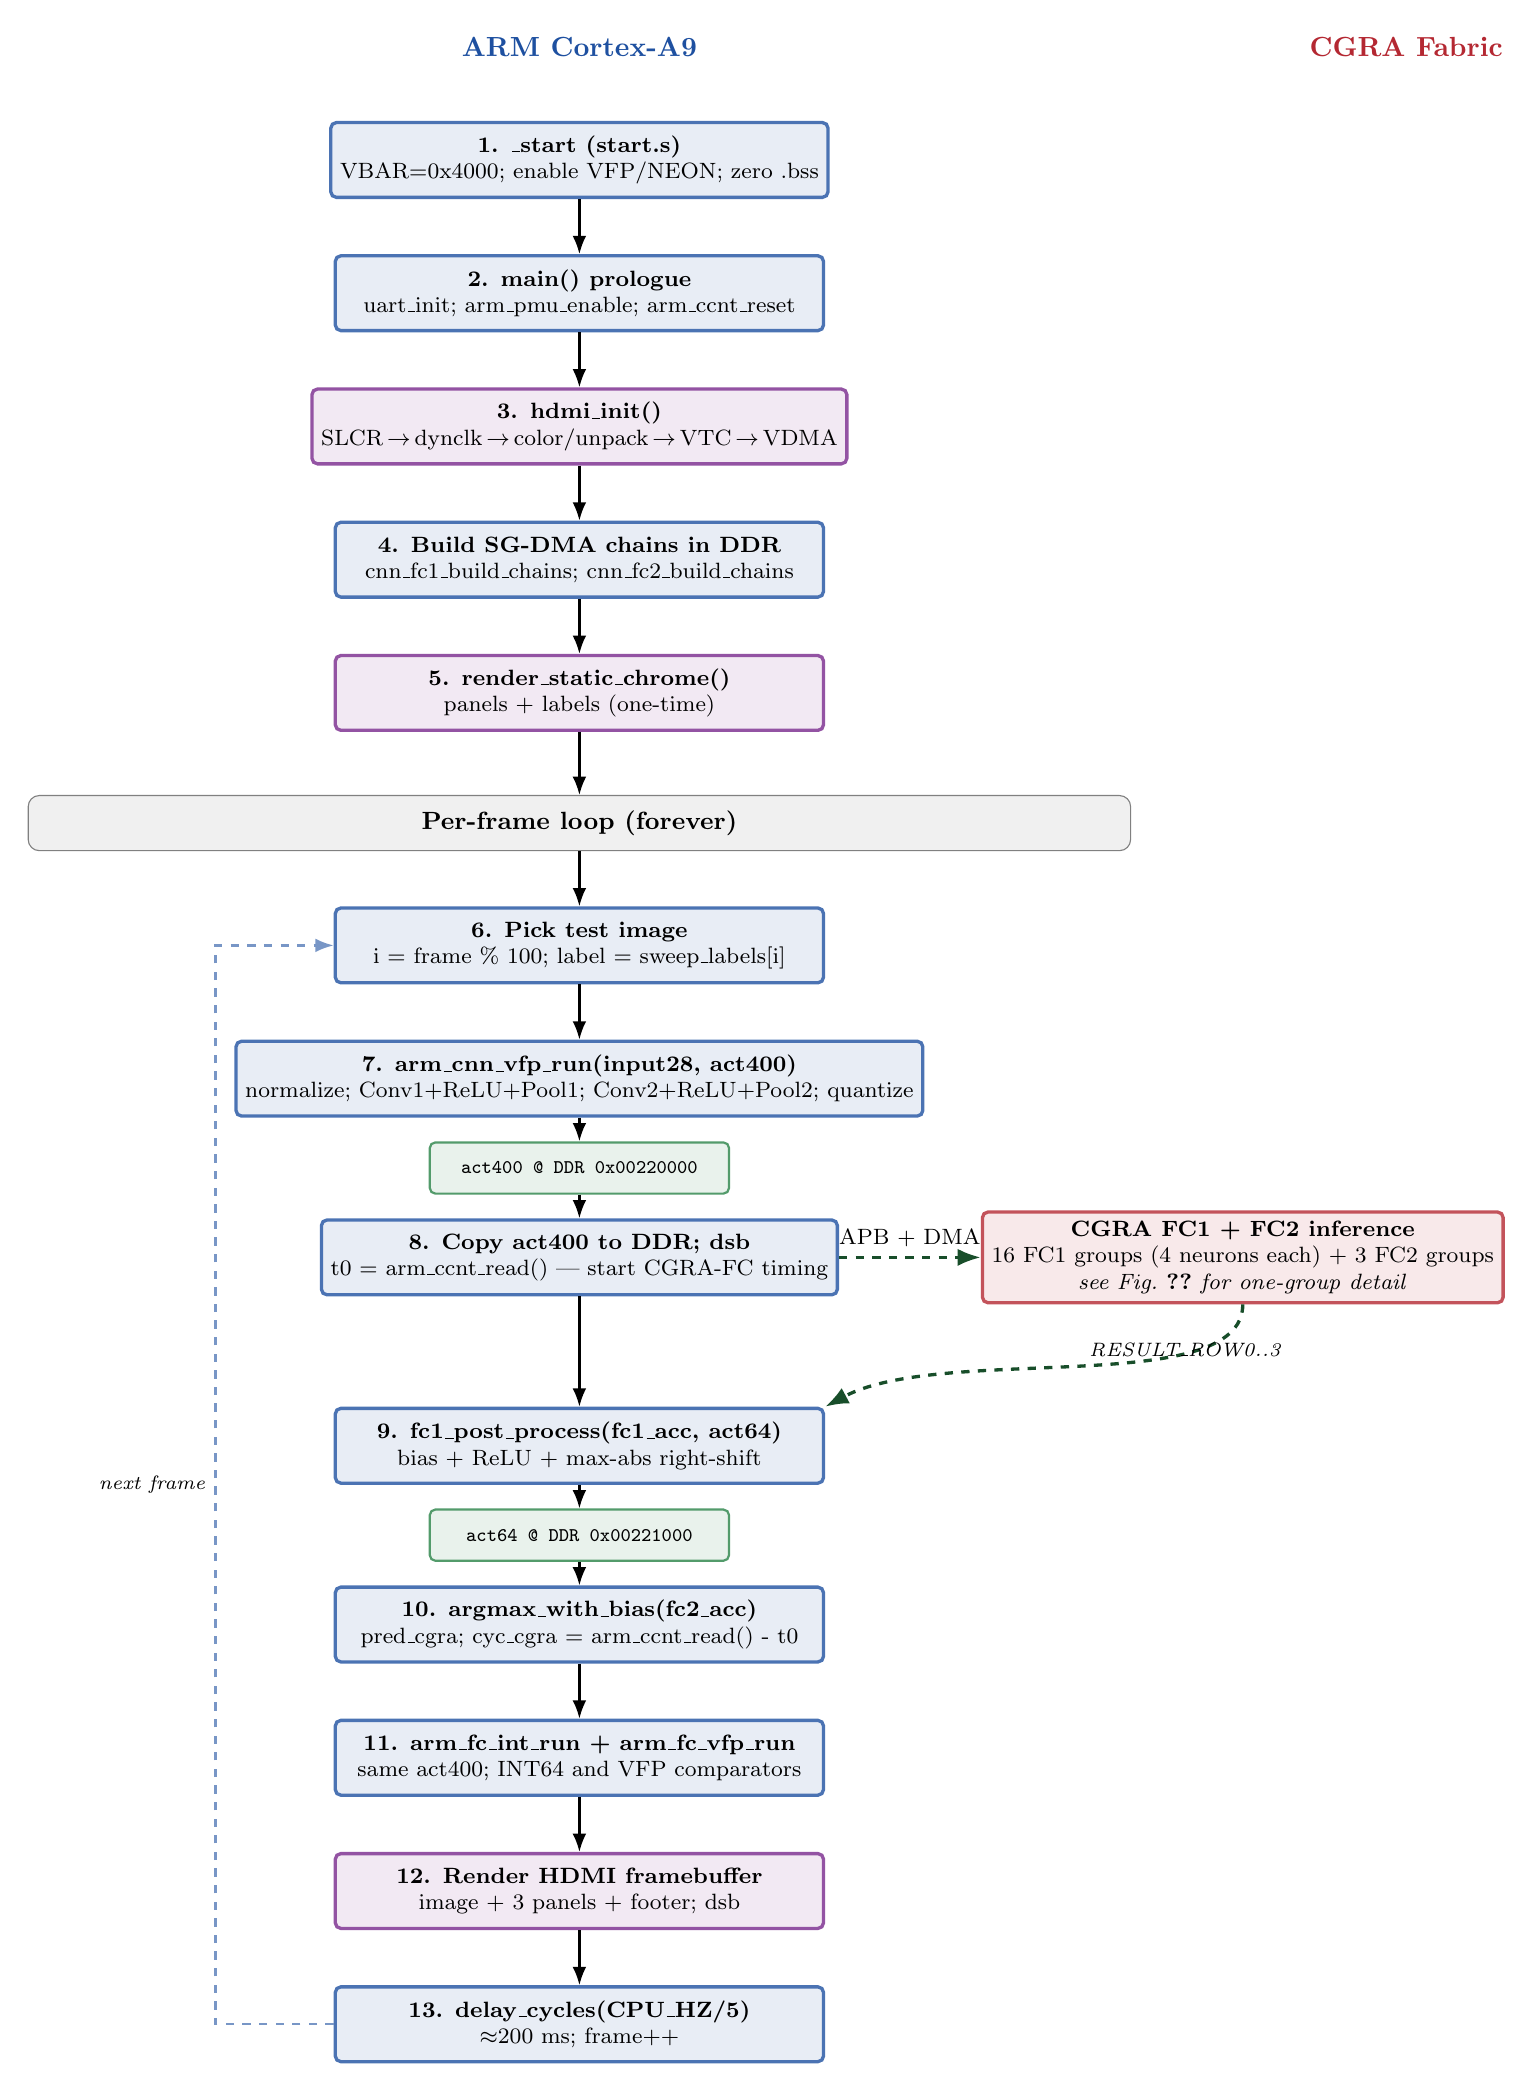
\begin{tikzpicture}[
    node distance = 7mm and 18mm,
    every node/.append style = {font=\footnotesize},
    armnode/.style  = {rectangle, draw=armblue!80, fill=armblue!10,
                       very thick, minimum width=6.2cm, minimum height=0.95cm,
                       align=center, rounded corners=2pt},
    cgranode/.style = {rectangle, draw=cgrared!80, fill=cgrared!10,
                       very thick, minimum width=6.2cm, minimum height=0.95cm,
                       align=center, rounded corners=2pt},
    hdminode/.style = {rectangle, draw=hdmipurple!80, fill=hdmipurple!10,
                       very thick, minimum width=6.2cm, minimum height=0.95cm,
                       align=center, rounded corners=2pt},
    ddrbox/.style   = {rectangle, draw=ddrgreen!80, fill=ddrgreen!10,
                       thick, minimum width=3.8cm, minimum height=0.65cm,
                       align=center, font=\scriptsize\ttfamily,
                       rounded corners=2pt},
    arrow/.style    = {-Latex, thick},
    handoff/.style  = {-Latex, very thick, dashed, draw=ddrgreen!60!black,
                       font=\scriptsize\itshape},
    looplbl/.style  = {rectangle, draw=black!50, fill=gray!12,
                       rounded corners=4pt, minimum width=14cm,
                       minimum height=0.7cm, font=\bfseries\small,
                       align=center}
]

% --- Lane titles ---
\node (armT)  at (0,0) [font=\bfseries] {\textcolor{armblue}{ARM Cortex-A9}};
\node (cgraT) at (10.5,0) [font=\bfseries] {\textcolor{cgrared}{CGRA Fabric}};

% --- Boot chain (ARM only) ---
\node[armnode, below=of armT]      (boot)     {\textbf{1. \_start (start.s)}\\
   VBAR=0x4000; enable VFP/NEON; zero .bss};
\node[armnode, below=of boot]      (prologue) {\textbf{2. main() prologue}\\
   uart\_init; arm\_pmu\_enable; arm\_ccnt\_reset};
\node[hdminode, below=of prologue] (hdmi)     {\textbf{3. hdmi\_init()}\\
   SLCR\,$\to$\,dynclk\,$\to$\,color/unpack\,$\to$\,VTC\,$\to$\,VDMA};
\node[armnode, below=of hdmi]      (chains)   {\textbf{4. Build SG-DMA chains in DDR}\\
   cnn\_fc1\_build\_chains; cnn\_fc2\_build\_chains};
\node[hdminode, below=of chains]   (chrome)   {\textbf{5. render\_static\_chrome()}\\
   panels + labels (one-time)};

% --- Loop header ---
\node[looplbl, below=8mm of chrome] (loop) {Per-frame loop (forever)};

% --- Per-frame chain (ARM) ---
\node[armnode, below=of loop]      (pick) {\textbf{6. Pick test image}\\
   i = frame \% 100; label = sweep\_labels[i]};
\node[armnode, below=of pick]      (vfp)  {\textbf{7. arm\_cnn\_vfp\_run(input28, act400)}\\
   normalize; Conv1+ReLU+Pool1; Conv2+ReLU+Pool2; quantize};
\node[ddrbox,  below=3mm of vfp]   (ddrA) {act400 @ DDR \texttt{0x00220000}};
\node[armnode, below=3mm of ddrA]  (kick) {\textbf{8. Copy act400 to DDR; dsb}\\
   t0 = arm\_ccnt\_read() --- start CGRA-FC timing};

% --- CGRA inset block (aligned to the right of the kick stage) ---
\node[cgranode, right=of kick] (cgrafc) {\textbf{CGRA FC1 + FC2 inference}\\
   16 FC1 groups (4 neurons each) + 3 FC2 groups\\
   \emph{see Fig.~\ref{fig:fc-group} for one-group detail}};

% --- Continuation on ARM ---
\node[armnode, below=14mm of kick]  (post)   {\textbf{9. fc1\_post\_process(fc1\_acc, act64)}\\
   bias + ReLU + max-abs right-shift};
\node[ddrbox,  below=3mm of post]   (ddrB)   {act64 @ DDR \texttt{0x00221000}};
\node[armnode, below=3mm of ddrB]   (argmax) {\textbf{10. argmax\_with\_bias(fc2\_acc)}\\
   pred\_cgra; cyc\_cgra = arm\_ccnt\_read() - t0};
\node[armnode, below=of argmax]     (others) {\textbf{11. arm\_fc\_int\_run + arm\_fc\_vfp\_run}\\
   same act400; INT64 and VFP comparators};
\node[hdminode, below=of others]    (render) {\textbf{12. Render HDMI framebuffer}\\
   image + 3 panels + footer; dsb};
\node[armnode, below=of render]     (delay)  {\textbf{13. delay\_cycles(CPU\_HZ/5)}\\
   $\approx$200 ms; frame++};

% --- Vertical flow arrows along the ARM column ---
\foreach \src/\dst in
   {boot/prologue, prologue/hdmi, hdmi/chains, chains/chrome,
    chrome/loop, loop/pick, pick/vfp, vfp/ddrA, ddrA/kick,
    kick/post, post/ddrB, ddrB/argmax, argmax/others,
    others/render, render/delay}
   \draw[arrow] (\src) -- (\dst);

% --- ARM <-> CGRA handoffs (only at well-defined boundaries) ---
\draw[handoff] (kick.east) -- node[above,sloped]{APB + DMA} (cgrafc.west);
\draw[handoff] (cgrafc.south) .. controls +(0,-12mm) and +(15mm,8mm) ..
   node[above right, font=\scriptsize\itshape]{RESULT\_ROW0..3} (post.north east);

% --- Loopback arrow on the left side ---
\draw[arrow, dashed, draw=armblue!60]
   (delay.west) -- ++(-15mm,0)
   |- node[pos=0.25, left, font=\scriptsize\itshape]{next frame} (pick.west);

\end{tikzpicture}%
}
\caption{Per-frame execution flow. Boot stages (top, above the labelled
bar) execute once; per-frame stages execute indefinitely. Blue
boxes are ARM-side, red boxes are CGRA-side, purple boxes are
HDMI-pipeline operations, and green mini-boxes mark DDR-resident handoff
buffers. Dashed green arrows are APB/DMA crossings of the ARM--CGRA
boundary. The CGRA-FC block expands to Fig.~\ref{fig:fc-group}.}
\label{fig:swimlane}
\end{figure}

The flowchart is hierarchical: the per-frame loop executes
indefinitely, while the boot stages run once. The CGRA is invoked
\emph{twice} per frame (FC1 and FC2), with the ARM core orchestrating
data movement and post-processing in between. The remainder of this
subsection walks through every numbered block; Figure~\ref{fig:fc-group}
then zooms into the internal six-step structure of one
\code{cnn\_fc\_run\_group()} call.

\paragraph{Boot phase (steps 1--5, executed once at power-on).}
\begin{enumerate}[leftmargin=2.1em, label=\textbf{Step \arabic*.},
                  itemsep=4pt, topsep=2pt]
\item \textbf{Reset vector in \file{start.s}.} On power-on the
Cortex-A9 starts execution at the reset vector. The hand-written
assembly sets the Vector Base Address Register (VBAR) to
\addr{00004000}, enables the VFP/NEON coprocessor (CPACR bits cp10
and cp11) and clears FPEXC, zeros the \code{.bss} section in OCM,
and finally jumps to the C \code{main()}. The MMU and the L1 data
cache are deliberately left disabled --- all subsequent memory
accesses are physical and uncached, which keeps the cycle-counter
measurements deterministic.

\item \textbf{\code{main()} prologue.} The first few statements of
\code{main()} bring up the host's instrumentation infrastructure.
\code{uart\_init()} configures the Zynq PS UART0 for 115200 baud, 8N1,
on MIO\,14/15. \code{arm\_pmu\_enable()} writes the Performance
Monitor Control Register (PMCR) to enable the on-chip cycle counter,
and \code{arm\_ccnt\_reset()} clears it so that all subsequent
\code{arm\_ccnt\_read()} calls return a monotonically-increasing
cycle count. Without these calls, the head-to-head FC timings would
be impossible.

\item \textbf{HDMI pipeline bring-up.} \code{hdmi\_init()} brings up
the five PL IPs that make up the video output. It first unlocks the
PS SLCR registers, sets FCLK0 to 100 MHz (the reference clock that
\code{axi\_dynclk} expects), re-locks SLCR, and then calls
\code{hdmi\_force\_idle()} to quench any leftover state from a prior
ELF run. It then programs the MMCM inside \code{axi\_dynclk} to
synthesize a 25.175 MHz pixel clock, loads an identity 3$\times$3
colour-matrix into \code{color\_convert}, sets \code{pixel\_unpack}
to the V\_24 (3-byte BGR) mode, programs \code{v\_tc} for 640$\times$480
@ 60 Hz timing, and finally arms \code{axi\_vdma} in MM2S mode
pointing at the framebuffer at \addr{1F000000}.

\item \textbf{Build SG-DMA descriptor chains in DDR.} The host now
calls \code{cnn\_fc1\_build\_chains()} followed by
\code{cnn\_fc2\_build\_chains()}. These two routines populate a
region of DDR with linked lists of \code{cgra\_sg\_dma\_descriptor\_t}
records --- one chain per phase of an FC group (SPM-preload, ACC\_CLR,
MAC-restore, east-readout, plus a one-time east-chain init). After
this step, dispatching a 64-neuron FC1 layer or a 10-neuron FC2
layer requires no further descriptor construction at run time; the
host simply writes a chain's head pointer into the
\reg{DMA\_DESC\_HEAD} register and asserts the chain-start bit.

\item \textbf{Render static chrome.} Finally, \code{render\_static\_chrome()}
paints the panel rectangles, the labels (``CGRA-FC'', ``ARM-INT-FC'',
``ARM-VFP-FC''), and the screen titles to the HDMI framebuffer. These
elements never change across frames, so they are written once at boot
rather than on each per-frame render pass. A single \code{dsb}
guarantees the writes have reached DDR before the VDMA's next scan-out
cycle picks them up.
\end{enumerate}

\paragraph{Per-frame phase (steps 6--13, repeated forever).}
\begin{enumerate}[leftmargin=2.1em, label=\textbf{Step \arabic*.}, start=6,
                  itemsep=4pt, topsep=2pt]
\item \textbf{Pick the next test image.} The host computes
\code{i = frame \% SWEEP\_N\_IMAGES} to index into the 100-image
fixture and looks up \code{label = sweep\_labels[i]} for accuracy
bookkeeping. Both arrays live in the read-only \code{.cnn\_sweep}
DDR section, so no copy is needed --- the ARM operates on
pointers directly into the fixture.

\item \textbf{ARM-VFP convolutional front-end.} The function
\code{arm\_cnn\_vfp\_run()} takes the raw \code{sweep\_input28[i]}
array as input and fills the output buffer \code{act400[400]} after
running the full floating-point convolutional pipeline on the ARM
core. Inside it,
\code{normalize\_input()} converts each \code{uint8\_t} pixel into a
VFPv3 float and applies the MNIST whitening transform; Conv1
(3$\times$3, 1$\to$8 channels) is computed in place; \code{relu\_inplace()}
clamps negatives to zero; \code{maxpool\_2x2()} reduces to 13$\times$13$\times$8;
the same Conv$+$ReLU$+$Pool sequence is repeated for Conv2 (3$\times$3,
8$\to$16); the 5$\times$5$\times$16 tensor is transposed from HWC to CHW order
to match PyTorch's flatten convention; and finally
\code{quantize\_to\_int32()} computes the per-image max-abs and
rescales the 400 values to the INT16 dynamic range required by FC1.
The output, \code{act400[400]}, is a stack-resident INT32 buffer.

\item \textbf{Stage the activation in DDR and start timing.} The host
copies \code{act400[400]} into the DDR-resident staging buffer at
\reg{ACT400\_DDR\,=\,0x00220000} using a simple C loop of volatile
INT32 writes. A \code{dsb} memory barrier flushes the ARM
write-buffer; without it, the CGRA's DMA engine could begin reading
DDR before the ARM's writes have actually landed. Then
\code{t0\,=\,arm\_ccnt\_read()} captures the starting cycle so the
CGRA-FC stage can be timed independently of the Conv stage above.

\item \textbf{CGRA executes FC1 and FC2.} This is the principal
ARM$\leftrightarrow$CGRA handoff. The host first calls
\code{cnn\_fc1\_tile\_preload(ACT400\_DDR)} which broadcasts the
1600-byte \code{act400} into all four CGRA tile banks via a single
1-D DMA transfer. It then iterates 16 times, once per output-neuron
group of four, calling \code{cnn\_fc1\_run\_group(g, \&fc1\_acc[g*4])}.
Each call triggers the six-step pre-built SG-DMA + CU sequence
detailed in Figure~\ref{fig:fc-group} (SPM preload, ACC\_CLR, MAC
restore, MAC CU run, east readout, APB drain) and produces four
INT32 dot products. The 64-element \code{fc1\_acc[]} array is then
post-processed (step~9), restaged in DDR, and the FC2 layer is
dispatched in the same way --- three groups instead of sixteen,
with the trailing two slots discarded since FC2 has only 10 outputs.

\item \textbf{FC1 post-processing on the ARM.} The 64 FC1 accumulator
values are passed to \code{fc1\_post\_process()}, which adds the
per-neuron bias from \code{mnist\_fc1\_bias\_q[]}, applies ReLU,
finds the maximum absolute value across all 64 outputs, and right-shifts
the entire buffer so that every value fits in INT16 range. The
shifted vector \code{act64[64]} is then staged in DDR at
\reg{ACT64\_DDR\,=\,0x00221000}, ready to feed FC2. This step
is too small (64 elements) to benefit from CGRA acceleration; the ARM
finishes it in well under one microsecond.

\item \textbf{Argmax and FC timing close.} After FC2 returns, the
host calls \code{argmax\_with\_bias(fc2\_acc)} which adds the
per-class bias from \code{mnist\_fc2\_bias\_q[]} to each of the ten
logits and returns the index of the maximum --- the predicted digit
class. \code{t1\,=\,arm\_ccnt\_read()} stops the timing window so
\code{cyc\_cgra\,=\,t1\,-\,t0} records exactly how many cycles the
FC stage consumed on the CGRA path.

\item \textbf{Re-time the same input on the two ARM-only comparators.}
The host now repeats the FC stage twice more, this time without the
CGRA: \code{arm\_fc\_int\_run(act400, cnn\_spm\_start)} executes the
same INT64-accumulator math entirely on the Cortex-A9 (matching the
CGRA's integer pipeline byte-for-byte), and
\code{arm\_fc\_vfp\_run(act400, cnn\_spm\_start)} executes the same
FC stage with VFPv3 floating-point MACs (the ``modern compiler
default'' comparator). Each run is wrapped in its own
\code{arm\_ccnt\_read()} window so the three timings are mutually
independent and directly comparable. All three paths see the same
input \code{act400}, so the only variable being measured is the FC
implementation itself.

\item \textbf{Render the result to HDMI.} \code{fbm\_draw\_image28()}
blits the raw 28$\times$28 input digit at 8$\times$ scale into a 224$\times$224
region of the framebuffer at the top of the screen.
\code{render\_panel()} then redraws each of the three result panels
with the latest \code{PRED}, \code{GT}, \code{$\mu$s}, and \code{FPS}
values; \code{render\_footer()} redraws the speedup ratios and the
three per-path accuracy counters. All of these primitives are simple
volatile writes into the DDR framebuffer; a final \code{dsb} ensures
the writes have drained before the VDMA's next scan-out pass.

\item \textbf{Inter-frame delay and loopback.}
\code{delay\_cycles(CPU\_HZ\,/\,5)} busy-waits for approximately
200 ms by polling the same PMU cycle counter used for the FC timing.
This dwell rate gives a defense audience roughly five frames per
second of visible inference, which is slow enough to read each
prediction comfortably and fast enough to convey live operation.
\code{frame++} and control returns to step~6 with the next image.
\end{enumerate}

\begin{figure}[!htbp]
\centering
\resizebox{0.92\textwidth}{!}{%
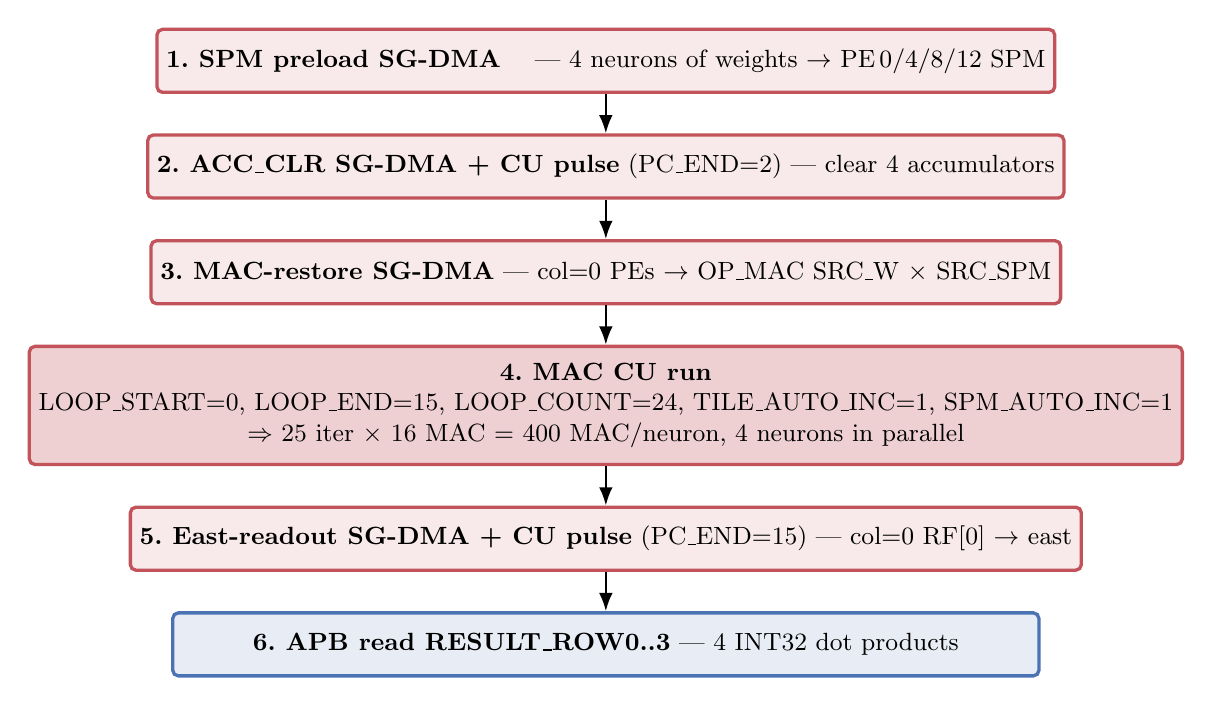
\begin{tikzpicture}[
   node distance = 5mm,
   every node/.append style = {font=\small},
   stepnode/.style = {rectangle, draw=cgrared!80, fill=cgrared!10,
                      very thick, minimum width=11cm, minimum height=0.8cm,
                      align=center, rounded corners=2pt},
   macstep/.style  = {rectangle, draw=cgrared!80, fill=cgrared!22,
                      very thick, minimum width=11cm, minimum height=1.5cm,
                      align=center, rounded corners=2pt},
   armstep/.style  = {rectangle, draw=armblue!80, fill=armblue!10,
                      very thick, minimum width=11cm, minimum height=0.8cm,
                      align=center, rounded corners=2pt},
   stepArrow/.style = {-Latex, thick}
]
\node[stepnode] (s1) {\textbf{1.\ SPM preload SG-DMA} \quad
   --- 4 neurons of weights $\to$ PE\,0/4/8/12 SPM};
\node[stepnode, below=of s1]  (s2)
   {\textbf{2.\ ACC\_CLR SG-DMA + CU pulse} (PC\_END=2) --- clear 4 accumulators};
\node[stepnode, below=of s2]  (s3)
   {\textbf{3.\ MAC-restore SG-DMA} --- col=0 PEs $\to$ OP\_MAC SRC\_W $\times$ SRC\_SPM};
\node[macstep,  below=of s3]  (s4)
   {\textbf{4.\ MAC CU run}\\
    LOOP\_START=0, LOOP\_END=15, LOOP\_COUNT=24,
    TILE\_AUTO\_INC=1, SPM\_AUTO\_INC=1\\
    $\Rightarrow$ 25 iter $\times$ 16 MAC = 400 MAC/neuron, 4 neurons in parallel};
\node[stepnode, below=of s4]  (s5)
   {\textbf{5.\ East-readout SG-DMA + CU pulse} (PC\_END=15) --- col=0 RF[0] $\to$ east};
\node[armstep,  below=of s5]  (s6)
   {\textbf{6.\ APB read RESULT\_ROW0..3} --- 4 INT32 dot products};
\foreach \a/\b in {s1/s2,s2/s3,s3/s4,s4/s5,s5/s6}
   \draw[stepArrow] (\a) -- (\b);
\end{tikzpicture}%
}
\caption{The six-step structure of one \code{cnn\_fc\_run\_group($g$)}
invocation. Steps 1--5 execute on the CGRA fabric without ARM
intervention; step 6 is the only APB read in the per-group critical
path. FC1 calls this 16 times per frame (64 outputs); FC2 calls it
3 times (10 outputs; last group has 2 valid neurons).}
\label{fig:fc-group}
\end{figure}

% =====================================================================
\section{Software Implementation}
\label{sec:ch4-impl}
% =====================================================================

\subsection{Initialization of Memory Regions}
\label{ssec:mmap}

In a Linux deployment the same address map would be accessed through
\code{mmap()} on \file{/dev/mem} or a UIO device node
(\code{open("/dev/uio0", O\_RDWR)} followed by
\code{mmap(..., PROT\_READ\,$|$\,PROT\_WRITE, MAP\_SHARED, fd, 0)}),
with the kernel translating between virtual and physical addresses.
In the present bare-metal deployment, however, the Cortex-A9 boots
with the MMU disabled and the L1 data cache off; all accesses are
physical and identity-mapped. Memory-mapped peripherals are accessed
by casting their physical addresses to \code{volatile uint32\_t *} and
dereferencing them directly. A single header, \file{cgra.h}, centralizes
the address constants and provides inline wrappers for register access
(\Cref{lst:cgra-h-base}).

\begin{lstlisting}[caption={Base addresses and register helpers for the
CGRA APB and DMA windows (excerpt from \file{cgra.h}).},
label={lst:cgra-h-base}]
#define CGRA_BASE          0x43C80000UL  /* APB base, PYNQ-base bolt-on */
#define CGRA_PFX_TILE      0x10000000UL  /* tile memory window         */
#define CGRA_PFX_CONFIG    0x20000000UL  /* per-PE config RAM window   */
#define CGRA_PFX_SPM       0x40000000UL  /* per-PE scratchpad window   */
#define CGRA_TILE_BCAST    (CGRA_PFX_TILE | 0x80000000UL)

static inline void cgra_wr(uint32_t off, uint32_t v) {
    *(volatile uint32_t *)(CGRA_BASE + off) = v;
}
static inline uint32_t cgra_rd(uint32_t off) {
    return *(volatile uint32_t *)(CGRA_BASE + off);
}
\end{lstlisting}

The CGRA's 30 APB control-status registers occupy offsets
\addr{00}--\addr{84} from \reg{CGRA\_BASE}; the application accesses
them exclusively through \code{cgra\_wr()}/\code{cgra\_rd()}. Three
additional address windows --- \reg{CGRA\_PFX\_TILE},
\reg{CGRA\_PFX\_CONFIG}, and \reg{CGRA\_PFX\_SPM} --- are \emph{not}
directly addressable from the ARM core. They are reachable only as
\emph{destinations} of the CGRA's integrated DMA engine; writing the
SPM, for instance, is accomplished by configuring the DMA with
\code{DMA\_DST = CGRA\_SPM\_PE\_ADDR(pe, 0)} and triggering a transfer.
This routing keeps the high-bandwidth weight and activation traffic
on the dedicated DMA path rather than serializing it through the
narrow APB bus.

The DDR layout is controlled by the linker script \file{linker\_cnn.ld}.
Three custom section attributes redirect large objects to specific DDR
regions so that on-chip memory (OCM, 120~KB) is reserved for code,
stack, and small \code{.bss} arrays:

\begin{itemize}[leftmargin=1.4cm,itemsep=2pt,topsep=2pt]
\item \code{.cnn\_spm} --- 105~KB FC weight blob at DDR \addr{00200000}.
\item \code{.cnn\_sweep} --- 78~KB test-image fixture at DDR \addr{00240000}.
\item \code{.cnn\_runtime} --- 105~KB float-weight cache (VFP comparator),
NOLOAD, at DDR \addr{00253CA0}.
\end{itemize}

Each large array in the source carries
\code{\_\_attribute\_\_((section(\dots)))} to be placed in the appropriate
region. The HDMI framebuffer is fixed at \addr{1F000000}
(640 $\times$ 480 $\times$ 3 bytes $=$ 921{,}600 bytes) by the VDMA
configuration; the ARM treats it as a flat array of BGR triplets.

\subsection{Initialization of Weights and CGRA Configuration}
\label{ssec:weights}

The CNN's weight tensors are produced offline by the Python
quantization pipeline (\file{07\_sw/cnn\_eval/quantize\_cgra.py}) and
exported as two binary blobs: \file{mnist\_weights\_conv.bin} (2.5~KB,
two Conv layers and their biases in INT16/INT32) and
\file{mnist\_weights\_spm.bin} (105~KB, FC1 and FC2 weights in
INT16-in-INT32 SPM layout). These are embedded into the ELF at
compile time using the assembler's \code{.incbin} directive
(\Cref{lst:incbin}).

\begin{lstlisting}[language={[x86masm]Assembler},caption={Weight-blob
embedding via the \code{.incbin} directive. The linker places these
sections at fixed DDR addresses.},label={lst:incbin}]
    .section .cnn_spm, "a"
    .global cnn_spm_start
cnn_spm_start:
    .incbin "../cnn_eval/mnist_weights_spm.bin"

    .section .cnn_conv_spm, "a"
    .global cnn_conv_start
cnn_conv_start:
    .incbin "../cnn_eval/mnist_weights_conv.bin"
\end{lstlisting}

At runtime, the host code references the blobs via the linker-emitted
symbols \code{cnn\_spm\_start} and \code{cnn\_conv\_start}; no file I/O
is required.

Configuration of the CGRA fabric proceeds at two levels. The
\emph{microarchitectural level} programs each PE's 16-slot context-memory
with a kernel-specific 64-bit instruction word (encoding opcode, two
source selectors, destination, route mask, and a 16-bit immediate).
The \emph{macroarchitectural level} programs the CU's loop-count
registers and auto-increment enables that govern how those PE contexts
are sequenced.

For PE configuration, the CGRA exposes a \textbf{Configuration Broadcaster}:
writing a 64-bit instruction word to the slot-0 address of any PE causes
an on-chip FSM to replay the same word into slots 1--15 of that PE within
15 cycles. To install a heterogeneous multi-slot kernel, the application
writes slot 0 first (broadcasting an idle value), then overwrites the
specific slots that require different instructions. For a 16-PE broadcast
(every PE programmed identically), bit 14 of the destination address
(\reg{CGRA\_CFG\_BCAST\_FLAG}) enables a second broadcast plane that
fans the write to all 16 PEs in parallel. The inline helper
\code{cgra\_config\_pe\_slot()} assembles the 64-bit word and issues the
double-pumped (\code{hi32}/\code{lo32}) APB-DMA pair that latches it into
the PE config RAM.

For the FC kernel the application takes advantage of a higher-level
abstraction: \code{cnn\_fc1\_build\_chains()} and
\code{cnn\_fc2\_build\_chains()} are called once at boot and pre-compute
a set of \textbf{Scatter-Gather DMA descriptors} in DDR, each describing
one phase of the FC group sequence:

\begin{itemize}[leftmargin=1.3cm,itemsep=2pt,topsep=2pt]
\item \textbf{SPM preload chain} --- loads four neurons' worth of weights
      into the col-0 PEs' scratchpads (per-group);
\item \textbf{ACC\_CLR chain} --- broadcasts the accumulator-clear opcode
      to all four col-0 PEs;
\item \textbf{MAC-restore chain} --- broadcasts the MAC opcode to the
      same col-0 PEs;
\item \textbf{East-readout chain} --- reprograms col-0 PEs to
      \code{PASS0\,SRC\_RF\,ROUTE\_E} for the result drain;
\item \textbf{East-chain init} (one-time) --- programs col-1/2/3 PEs to
      \code{PASS0\,SRC\_W\,ROUTE\_E}, forming the east-bound result
      conveyor.
\end{itemize}

Each chain is a linked list of \code{cgra\_sg\_dma\_descriptor\_t}
records:

\begin{lstlisting}[caption={SG-DMA descriptor layout used by the FC chain
infrastructure (from \file{cgra.h}).},label={lst:sgdma-desc}]
typedef struct {
    uint32_t src;        /* DDR source address                  */
    uint32_t dst;        /* CGRA destination (config/SPM/tile)  */
    uint32_t size;       /* byte count                          */
    uint32_t next_ptr;   /* DDR pointer to next descriptor,     */
                         /* or 0 to terminate the chain          */
} cgra_sg_dma_descriptor_t;
\end{lstlisting}

At runtime, dispatching a full FC group requires no further configuration
of the PE fabric: the application writes the head pointer of the
appropriate chain to \reg{DMA\_DESC\_HEAD} and asserts \reg{DMA\_CTRL}
bit 1; the chain controller fetches each descriptor, executes the
transfer, and follows \code{next\_ptr} until termination. This
pre-built-chain pattern reduces the per-frame APB write count from
several hundred to fewer than fifty, and is the dominant reason the
CGRA-FC stage completes in 1.50~ms on silicon.

\subsection{Reading Input Data}
\label{ssec:input}

For the MNIST demo the input dataset is embedded into the ELF,
eliminating any runtime I/O dependency. The Python utility
\file{07\_sw/cnn\_eval/emit\_sweep\_fixture.py} selects 100
representative test images from the MNIST test set, exports their
28$\times$28 grayscale pixel arrays as a single C header file
\file{mnist\_sweep\_fixture.h}, and tags the arrays with the
\code{SWEEP\_RODATA} section attribute (\Cref{lst:sweep}).

\begin{lstlisting}[caption={Test fixture, auto-generated.  Linker places
the 78~KB array at DDR \addr{00240000}.},label={lst:sweep}]
#define SWEEP_RODATA __attribute__((section(".cnn_sweep")))
static const uint8_t SWEEP_RODATA sweep_input28[100][784] = { ... };
static const uint8_t SWEEP_RODATA sweep_labels[100]       = { ... };
\end{lstlisting}

At each frame the application indexes into these arrays with
\code{i = frame \% 100}, obtaining \code{sweep\_input28[i]} (the raw
\code{uint8\_t[784]} pixel buffer) and \code{sweep\_labels[i]} (the
ground-truth class for accuracy bookkeeping). Because the data resides
in DDR rather than OCM, no copy is required to make it accessible to
the ARM core; the \code{arm\_cnn\_vfp\_run()} entry point receives a
\code{const uint8\_t *} pointer directly into the read-only blob.

The activation buffers consumed by the FC stage are allocated at
fixed DDR addresses by the application, not by the linker, so that
their physical addresses can be programmed directly into the CGRA
DMA's \reg{DMA\_SRC} register without requiring an inverse
virtual-to-physical lookup. Two such buffers suffice:

\begin{lstlisting}[caption={Fixed DDR staging addresses for inter-layer
activations (from the demo source).},label={lst:staging}]
#define ACT400_DDR  0x00220000UL  /* int32[400] act400 between Conv and FC1 */
#define ACT64_DDR   0x00221000UL  /* int32[64]  act64  between FC1 and FC2  */
\end{lstlisting}

These addresses sit in the gap between the \code{.cnn\_spm} section
(which ends at \addr{00219A00}) and the \code{.cnn\_sweep} section
(which begins at \addr{00240000}), leaving them safely outside any
linker-managed region.

\subsection{Preprocessing of Input Data}
\label{ssec:preprocess}

The pixel values in \code{sweep\_input28[i]} are unsigned 8-bit integers
in the range $[0, 255]$; the trained CNN expects normalized
floating-point inputs in the form $(v/255 - \mu)/\sigma$ with
$\mu = 0.1307$ and $\sigma = 0.3081$ (the standard MNIST whitening
parameters). The ARM-side preprocessing routine, implemented in
\file{arm\_cnn\_bm.c::normalize\_input()}, applies the transformation
in a tight VFP loop (\Cref{lst:normalize}).

\begin{lstlisting}[caption={Pixel normalization with VFPv3 hard-float.},label={lst:normalize}]
static void normalize_input(const uint8_t *src, float *dst)
{
    const float inv255 = 1.0f / 255.0f;
    const float mean   = 0.1307f;
    const float stdinv = 1.0f / 0.3081f;
    for (int i = 0; i < 784; ++i)
        dst[i] = ((float)src[i] * inv255 - mean) * stdinv;
}
\end{lstlisting}

The output \code{dst[]} is a 32-bit float array of length 784, populated
by VFPv3 single-cycle MAC instructions emitted by GCC under the
\code{-mfpu=vfpv3 -mfloat-abi=hard} flag combination. This vector then
feeds the two convolutional layers, each followed by a ReLU activation
and a 2$\times$2 max-pool, yielding successively the 26$\times$26$\times$8,
13$\times$13$\times$8, 11$\times$11$\times$16, and 5$\times$5$\times$16
feature tensors.

The output of the convolutional front-end is in floating point and in
HWC memory order. To match the input format expected by FC1 ---
a single 400-element integer activation vector in INT16 dynamic range
and in CHW order, mirroring the PyTorch tensor-flatten convention
against which the FC weights were trained --- two further preprocessing
steps are required. First, a \textbf{transpose} rearranges the
5$\times$5$\times$16 tensor from HWC to CHW order. Second, a
\textbf{per-image symmetric quantization} computes
$\text{max\_abs} = \max(|x|)$ over the 400 elements and rescales each
element to fit into INT16 (\Cref{lst:quantize}).

\begin{lstlisting}[caption={Per-image quantization producing the FC1
input vector \code{act400}.},label={lst:quantize}]
float inv_scale = 32767.0f / max_abs;
for (int i = 0; i < 400; ++i) {
    float q = buf_pool2_chw[i] * inv_scale;
    int32_t qi = (int32_t)(q >= 0.0f ? q + 0.5f : q - 0.5f);
    if (qi >  32767) qi =  32767;
    if (qi < -32768) qi = -32768;
    act400_out[i] = qi;
}
\end{lstlisting}

The resulting \code{act400[]} array is composed of 32-bit signed integers
whose values lie in $[-32{,}768, +32{,}767]$ --- i.e., they are
INT16-valued but stored in INT32 containers to match the CGRA
tile-memory data width. This per-image scaling means the absolute
magnitude of the activations is data-dependent, but their dynamic
range is fixed; this property is critical for keeping the downstream
INT16 $\times$ INT32 FC MAC accumulators inside the 40-bit CGRA
saturation envelope.

\subsection{Hardware Control: APB and DMA Subsystems}
\label{ssec:hwctrl}

After preprocessing, the host transfers \code{act400[]} into DDR at
the fixed staging address \reg{ACT400\_DDR}, issues an explicit Data
Synchronization Barrier
(\code{asm volatile("dsb" ::: "memory")}) to ensure the writes have
drained from the write-buffer into DDR, and then begins the CGRA
invocation sequence.

The CGRA exposes its full operating state through the APB CSR file.
\Cref{tab:regmap} summarizes the registers exercised by the FC inference
loop; the full 30-register map appears in Chapter~3.

\begin{table}[H]
\centering
\caption{CGRA APB registers exercised by the MNIST FC inference loop.
Offsets are from \reg{CGRA\_BASE = 0x43C80000}.}
\label{tab:regmap}
\small
\begin{tabularx}{\textwidth}{l l l X}
\toprule
\textbf{Offset} & \textbf{Mnemonic} & \textbf{R/W} & \textbf{Function in the FC loop} \\
\midrule
\addr{00} & \reg{DMA\_CTRL}        & W & \code{[0]=1}: start 1-D DMA; \code{[1]=1}: start SG-DMA chain. \\
\addr{04} & \reg{DMA\_STATUS}      & R & \code{[0]=1}: busy; \code{[1]=1}: done. \\
\addr{08} & \reg{DMA\_SRC}         & W & Source physical address. \\
\addr{0C} & \reg{DMA\_DST}         & W & Destination address (window-encoded). \\
\addr{10} & \reg{DMA\_SIZE}        & W & Byte count for 1-D transfer. \\
\addr{14} & \reg{DMA\_SRC\_STRIDE} & W & Cleared to 0 for 1-D transfers. \\
\addr{18} & \reg{DMA\_ROWS}        & W & Cleared to 0 for 1-D transfers. \\
\addr{1C} & \reg{DMA\_COLS}        & W & Cleared to 0 for 1-D transfers. \\
\addr{20} & \reg{CU\_CTRL}         & W & \code{[0]=1}: start CU; \code{[1]=1}: soft-reset CU. \\
\addr{24} & \reg{CU\_STATUS}       & R & \code{[0]=1}: busy; \code{[1]=1}: done. \\
\addr{3C} & \reg{CU\_PC\_END}      & W & Last slot the CU will execute before signalling done. \\
\addr{40} & \reg{RESULT\_DATA}     & R & Result FIFO front (PE(3,3) east port). \emph{Unused by the FC demo.} See note below. \\
\addr{48} & \reg{LOOP\_START}      & W & First slot of the hardware loop body. \\
\addr{4C} & \reg{LOOP\_END}        & W & Last slot of the hardware loop body. \\
\addr{50} & \reg{LOOP\_COUNT}      & W & Loop iteration count (inclusive). \\
\addr{58} & \reg{RESULT\_ROW0}     & R & Latched east-edge output of row 0 (PE 0--3). \\
\addr{5C} & \reg{RESULT\_ROW1}     & R & Latched east-edge output of row 1 (PE 4--7). \\
\addr{60} & \reg{RESULT\_ROW2}     & R & Latched east-edge output of row 2 (PE 8--11). \\
\addr{64} & \reg{RESULT\_ROW3}     & R & Latched east-edge output of row 3 (PE 12--15). \\
\addr{74} & \reg{TILE\_BANK\_SEL}  & W & Active tile bank (0--3). \\
\addr{78} & \reg{TILE\_AUTO\_INC}  & W & \code{[0]=1}: tile read addr advances by 16 each loop iter. \\
\addr{7C} & \reg{DMA\_DESC\_HEAD}  & W & SG-DMA chain head pointer (DDR-resident). \\
\addr{84} & \reg{SPM\_AUTO\_INC}   & W & \code{[0]=1}: SPM read offset advances by 16 each loop iter. \\
\bottomrule
\end{tabularx}
\small\par\vspace{0.4em}
\emph{Note on \reg{RESULT\_DATA}:} this FIFO is fed by the east port
of PE(3,3) every cycle and is the readout channel of the deprecated
per-pixel \code{cnn\_conv3x3\_pixel()} Conv kernel. The FC demo reads
\reg{RESULT\_ROW0..3} exclusively; \reg{RESULT\_DATA} is documented
here for completeness but is not exercised by the locked demo.
\end{table}

A single 1-D DMA transfer is initiated by writing the source,
destination, the three zeroed 2-D-mode registers, the byte count, and
finally asserting \reg{DMA\_CTRL} bit 0. The application then polls
\reg{DMA\_STATUS} bit 1 until it sets (\Cref{lst:cgra-dma}). The
explicit zeroing of the strided-mode registers is required because
the same register file serves both 1-D and 2-D transfers; failing to
clear them would re-issue the previous transfer's 2-D shape on top of
the new source/destination, producing partial writes.

\begin{lstlisting}[caption={1-D DMA helpers used by the FC
tile-preload step (excerpt from \file{cgra.h}).},label={lst:cgra-dma}]
static inline void cgra_dma_start(uint32_t src, uint32_t dst, uint32_t bytes)
{
    cgra_wr(CGRA_DMA_SRC,        src);
    cgra_wr(CGRA_DMA_DST,        dst);
    cgra_wr(CGRA_DMA_SRC_STRIDE, 0u);   /* disarm 2-D mode */
    cgra_wr(CGRA_DMA_ROWS,       0u);
    cgra_wr(CGRA_DMA_COLS,       0u);
    cgra_wr(CGRA_DMA_SIZE,       bytes);
    cgra_wr(CGRA_DMA_CTRL,       1u);   /* trigger */
}

static inline int cgra_dma(uint32_t src, uint32_t dst, uint32_t bytes)
{
    cgra_dma_start(src, dst, bytes);
    return cgra_dma_wait(1000000u);     /* poll DMA_STATUS bit 1 */
}
\end{lstlisting}

The DMA destination address encodes the target memory region.
Bits \code{[31:28]} select between DDR (\code{0x0}), tile memory
(\code{0x1}), PE configuration RAM (\code{0x2}), and per-PE scratchpad
(\code{0x4}). For tile broadcast --- writing the same 16 words to all
four tile banks in a single transfer --- bit 31 of the destination is
set, producing the \reg{CGRA\_TILE\_BCAST = 0x90000000} alias. The full
activation preload at the start of each FC inference is therefore the
single call \code{cgra\_dma(ACT400\_DDR, CGRA\_TILE\_BCAST, 1600)}.

The CU's hardware loop is the engine of the dense-matmul pattern.
With \reg{LOOP\_START} = 0, \reg{LOOP\_END} = 15,
\reg{LOOP\_COUNT} = 24, \reg{TILE\_AUTO\_INC} = 1, and
\reg{SPM\_AUTO\_INC} = 1, the CU executes 25 iterations of the 16-slot
PE program; each iteration advances the tile read address by 16 words
and the SPM read address by 16 words. The accumulator in each of the
four col-0 PEs (PE 0, 4, 8, 12) integrates
$25 \times 16 = 400$ weight-activation products --- exactly the dot
product required for one FC1 neuron. Four PEs execute four neurons in
parallel; one group therefore produces four FC1 outputs per CU
invocation, with no host involvement during the 25-iteration MAC loop.

Polling is preferred over interrupt-driven completion for two reasons.
First, the per-group CU completion time is approximately 60{,}000 cycles
($\approx 90$~$\mu$s at 666~MHz), and the entire FC1+FC2 stage --- sixteen
FC1 groups, three FC2 groups, plus inter-group SG-DMA orchestration ---
completes in roughly 1.00 million cycles (1.50~ms), well below any
meaningful timer-interrupt period. Polling adds no measurable latency on
this workload. Second, polling is deterministic in cycle count, whereas
the Cortex-A9 interrupt entry cost varies with the current pipeline
state. For a thesis whose central performance claim is a sub-millisecond
cycle-accurate measurement, deterministic timing of the wait loops is
preferable to a marginally lower mean latency.

\subsection{Output Layers and HDMI Display}
\label{ssec:output}

After the second FC group sequence terminates, the application reads
ten 32-bit signed integers from \reg{RESULT\_ROW0}--\reg{RESULT\_ROW3}
across three CU invocations (with the final two slots discarded). These
ten values are the unbiased FC2 logits in the CGRA's saturated INT32
accumulator scale. The final output layer of the network --- bias
addition and argmax --- is implemented in pure C on the ARM
(\Cref{lst:argmax}). A softmax is not strictly required because argmax
is invariant under any monotonically increasing function of the
logits; the final classification result is identical to that of a
softmax pipeline.

\begin{lstlisting}[caption={Final classification on the ARM
(verbatim from the demo source).},label={lst:argmax}]
static int argmax_with_bias(const int32_t fc2_acc[10])
{
    int32_t v[10];
    for (int i = 0; i < 10; ++i)
        v[i] = fc2_acc[i] + mnist_fc2_bias_q[i];
    int best = 0;
    for (int i = 1; i < 10; ++i)
        if (v[i] > v[best]) best = i;
    return best;
}
\end{lstlisting}

The FC1$\rightarrow$FC2 boundary does require a non-trivial
post-processing step (\code{fc1\_post\_process()}): for each of the
64 FC1 accumulator values, a bias from \code{mnist\_fc1\_bias\_q[]} is
added, a ReLU is applied, and the resulting buffer is requantized to
INT16 range via a max-abs right-shift so that downstream FC2 MACs remain
inside the INT32 envelope (\Cref{lst:fc1post}). This step is computed
on the ARM in a single 64-element loop and consumes a negligible
fraction of the inference time.

\begin{lstlisting}[caption={FC1$\rightarrow$FC2 post-processing
(verbatim from the demo source).},label={lst:fc1post}]
static void fc1_post_process(const int32_t fc1_acc[64], int32_t act64_out[64])
{
    int32_t tmp[64];
    int32_t max_abs = 0;
    for (int n = 0; n < 64; ++n) {
        int64_t s = (int64_t)fc1_acc[n] + (int64_t)mnist_fc1_bias_q[n];
        if (s < 0) s = 0;
        if (s > 0x7FFFFFFFLL) s = 0x7FFFFFFFLL;
        tmp[n] = (int32_t)s;
        if (tmp[n] > max_abs) max_abs = tmp[n];
    }
    int shift = 0;
    while ((max_abs >> shift) > 32767 && shift < 31) shift++;
    for (int n = 0; n < 64; ++n) act64_out[n] = tmp[n] >> shift;
}
\end{lstlisting}

The predicted class label, together with the ground-truth label, the
cycle-counter measurement, and the running accuracy total, are then
rendered to the HDMI framebuffer at \addr{1F000000}. The display geometry
places a 224$\times$224 upscaled rendering of the input digit at the top
of the 640$\times$480 frame, three result panels (CGRA-FC, ARM-INT-FC,
ARM-VFP-FC) directly below, and a footer with the live speedup ratios
and per-path accuracy counters.

Three primitives from \file{fb\_lib\_bm.c} suffice for the rendering:
\code{fbm\_draw\_image28(x0, y0, img784, scale)} writes a
\code{scale}$\times$\code{scale} block of identical-luminance pixels
for each of the 784 source bytes, producing the upscaled digit at any
integer magnification; \code{fbm\_draw\_text(x, y, s, fg, scale)}
walks a null-terminated ASCII string and rasterizes each character
through a compact $5\times7$ bitmap font; and
\code{hdmi\_rect(x, y, w, h, rgb)} clears the panel backgrounds and
footer region at the start of each frame.

Because the Cortex-A9 data cache is disabled in this bare-metal
configuration, every store to the framebuffer goes directly to DDR
and is observable by the AXI-VDMA on its next scan-out cycle without
any explicit cache flush. A single \code{dsb} instruction at the end
of the rendering block guarantees the AXI-VDMA reads a consistent
frame; the VDMA's free-running MM2S engine then drives the
pixel-unpack and color-convert IPs at 25.175~MHz to produce the
640$\times$480 @ 60~Hz HDMI signal.

The complete per-frame software cycle --- input read, ARM-VFP
Conv$+$Pool, three FC-path invocations, post-processing, and rendering
--- completes in approximately 35~ms of wall-clock work, of which the
three FC paths account for 1.50~ms, 5.60~ms, and 4.36~ms respectively.
A 200~ms inter-frame delay implemented with
\code{delay\_cycles(CPU\_HZ / 5)} reduces the user-visible refresh
rate to a comfortable 5~Hz, allowing a defense audience to observe
each prediction and the speedup numbers without strobing.

\Cref{tab:perf} summarizes the silicon measurements from the locked
demo. The CGRA's 3.74$\times$ wall-clock speedup over scalar-INT ARM
on identical math (both INT16 weights $\times$ INT32 activations into
INT64 accumulators) is the central performance claim of this thesis;
the 2.91$\times$ speedup over the hardware-VFP comparator is the
``honest asterisk'' that the same speedup holds even against a
modern compiler's default optimization target.

\begin{table}[H]
\centering
\caption{Silicon-measured performance of the three FC paths on the
locked demo, 201 frames sampled. PYNQ-Z2, Cortex-A9 @ 666~MHz, CGRA
@ 50~MHz.}
\label{tab:perf}
\small
\begin{tabular}{l c c c c}
\toprule
\textbf{Path} & \textbf{Per-image} & \textbf{FPS} & \textbf{Accuracy} & \textbf{Speedup vs CGRA} \\
\midrule
\textbf{CGRA-FC}   & \textbf{1.50 ms} & \textbf{668} & 195/201 (97.0\%) & --- (baseline) \\
ARM-INT-FC         & 5.60 ms         & 178          & 195/201 (97.0\%) & 0.27$\times$ \\
ARM-VFP-FC         & 4.36 ms         & 230          & 201/201 (100\%)  & 0.34$\times$ \\
\bottomrule
\end{tabular}
\end{table}

\Cref{tab:perf} compares the CGRA against a scalar ARM baseline. A
later silicon build (2026-06-03) re-ran the FC stage with the ARM path
compiled at \texttt{-O3 -mfpu=neon} and the CGRA compute time isolated
via its \code{CU\_CYCLES} counter, bounding the result against the
strongest software baseline: \textbf{131.5~$\mu$s} (CGRA compute) versus
\textbf{459~$\mu$s} (NEON Cortex-A9) --- a \textbf{3.5$\times$}
matched-compiler speedup, equivalently \textbf{$47\times$ per clock} at
$1/13$ the frequency. The roofline interpretation is given in Chapter~5.

This concludes the per-frame loop; control returns to the
``pick test image'' stage of \Cref{fig:swimlane} and the next input
image is processed.

% =====================================================================
% End of Chapter 4 content
% =====================================================================
 into the
% master thesis file and reuse preamble.tex's package set.
%
% Build:   latexmk -pdf main.tex
% Cleanup: latexmk -C

\documentclass[12pt,a4paper,oneside]{article}

% preamble.tex — packages, styles, and macros shared by main.tex
% Compile with: latexmk -pdf main.tex
% Tested with TeX Live 2023, pdflatex engine.

% --------------------------------------------------------------------
% Document class is set by main.tex; everything below is loaded after.
% --------------------------------------------------------------------

% ---- Encoding and language -----------------------------------------
\usepackage[utf8]{inputenc}
\usepackage[T1]{fontenc}
\usepackage{lmodern}
\usepackage[english]{babel}
\usepackage{microtype}

% ---- Page geometry -------------------------------------------------
\usepackage[a4paper,top=2.5cm,bottom=2.5cm,left=3cm,right=2.5cm]{geometry}
\usepackage{parskip}
\setlength{\parskip}{0.5em}

% Relax line-breaking so monospace identifiers and dense code-style
% paragraphs don't trigger overfull boxes. emergencystretch allows
% additional stretch on the last attempt; tolerance bumps the
% acceptable badness threshold.
\setlength{\emergencystretch}{3em}
\tolerance=1500
\hbadness=10000

% ---- Math / symbols ------------------------------------------------
\usepackage{amsmath,amssymb,amsthm}
\usepackage{textcomp}

% ---- Cross-references and links -----------------------------------
% NOTE: hyperref and cleveref must be loaded AFTER `listings` so cleveref
% can auto-detect the `lstlisting` counter. The `\usepackage{listings}`
% line is moved up to the Code-listings block below this one.
\usepackage[hidelinks,colorlinks=false]{hyperref}

% ---- Floats, tables, captions -------------------------------------
\usepackage{float}
\usepackage{booktabs}
\usepackage{array}
\usepackage{tabularx}
\usepackage{longtable}
\usepackage{multirow}
\usepackage[font=small,labelfont=bf,format=plain,justification=centering]{caption}
\usepackage{subcaption}
\usepackage{enumitem}

% ---- Colors --------------------------------------------------------
\usepackage{xcolor}
\definecolor{armblue}{RGB}{30,80,160}
\definecolor{cgrared}{RGB}{180,40,50}
\definecolor{ddrgreen}{RGB}{40,130,70}
\definecolor{hdmipurple}{RGB}{120,40,140}
\definecolor{codebg}{RGB}{245,245,248}
\definecolor{codeframe}{RGB}{200,200,210}
\definecolor{codecomment}{RGB}{60,120,60}
\definecolor{codekeyword}{RGB}{160,30,140}
\definecolor{codestring}{RGB}{180,80,30}
\definecolor{codenum}{RGB}{120,120,120}

% ---- Code listings -------------------------------------------------
% Loaded HERE (before cleveref) so cleveref sees the lstlisting counter.
\usepackage{listings}
\usepackage[capitalise,noabbrev]{cleveref}
\crefname{lstlisting}{Listing}{Listings}
\Crefname{lstlisting}{Listing}{Listings}
\lstdefinestyle{cstyle}{
    language=C,
    basicstyle=\ttfamily\footnotesize,
    keywordstyle=\color{codekeyword}\bfseries,
    commentstyle=\color{codecomment}\itshape,
    stringstyle=\color{codestring},
    numberstyle=\tiny\color{codenum},
    backgroundcolor=\color{codebg},
    rulecolor=\color{codeframe},
    showstringspaces=false,
    breaklines=true,
    breakatwhitespace=true,
    frame=single,
    framesep=4pt,
    numbers=left,
    numbersep=8pt,
    captionpos=b,
    xleftmargin=12pt,
    morekeywords={uint8_t,uint16_t,uint32_t,uint64_t,int8_t,int16_t,int32_t,int64_t,size_t,asm,volatile}
}
\lstset{style=cstyle}

% ---- TikZ ---------------------------------------------------------
\usepackage{tikz}
\usetikzlibrary{
    arrows.meta,
    calc,
    chains,
    decorations.pathmorphing,
    fit,
    positioning,
    shapes.geometric,
    shapes.symbols,
    backgrounds,
    shadows.blur
}

% TikZ styles for the swim-lane flowchart in Section 4.2.
\tikzset{
    armnode/.style    = {rectangle, draw=armblue!80, fill=armblue!10, very thick,
                         minimum width=5.5cm, minimum height=0.9cm, align=center,
                         font=\small, rounded corners=2pt},
    cgranode/.style   = {rectangle, draw=cgrared!80, fill=cgrared!10, very thick,
                         minimum width=5.5cm, minimum height=0.9cm, align=center,
                         font=\small, rounded corners=2pt},
    ddrbox/.style     = {rectangle, draw=ddrgreen!80, fill=ddrgreen!10, thick,
                         minimum width=2.4cm, minimum height=0.7cm, align=center,
                         font=\scriptsize, rounded corners=2pt},
    hdminode/.style   = {rectangle, draw=hdmipurple!80, fill=hdmipurple!10, very thick,
                         minimum width=5.5cm, minimum height=0.9cm, align=center,
                         font=\small, rounded corners=2pt},
    decision/.style   = {diamond, draw=armblue!80, fill=armblue!10, very thick,
                         aspect=2, inner sep=1pt, minimum width=4cm, font=\small,
                         align=center},
    arrow/.style      = {->, >=Latex, thick},
    handoff/.style    = {->, >=Latex, very thick, dashed, draw=ddrgreen!70!black},
    lanetitle/.style  = {font=\bfseries\large, align=center},
    lanebox/.style    = {rectangle, draw=gray!50, fill=gray!5, thick, rounded corners=4pt}
}

% ---- Convenience macros -------------------------------------------
\newcommand{\file}[1]{\texttt{\small #1}}
\newcommand{\reg}[1]{\texttt{\small #1}}
\newcommand{\code}[1]{\texttt{\small #1}}
\newcommand{\addr}[1]{\texttt{\small 0x#1}}

% Standard fixed widths for the register-map table.
\newcolumntype{R}[1]{>{\raggedright\arraybackslash}p{#1}}


% Section depth and numbering depth for a 1-chapter standalone build:
% start with section level (4.1, 4.2, ...) by re-numbering manually.
\renewcommand{\thesection}{4.\arabic{section}}
\renewcommand{\thesubsection}{4.\arabic{section}.\arabic{subsection}}
\renewcommand{\thesubsubsection}{4.\arabic{section}.\arabic{subsection}.\arabic{subsubsection}}
\renewcommand{\thefigure}{4.\arabic{figure}}
\renewcommand{\thetable}{4.\arabic{table}}
% Listings counter is created on first use by the `listings` package;
% renumber it via \AtBeginDocument so the counter exists at that point.
\AtBeginDocument{\renewcommand{\thelstlisting}{4.\arabic{lstlisting}}}

\title{\textbf{Chapter 4 — Software Design and Implementation} \\[0.3em]
       \large CGRA-Accelerated MNIST CNN Inference on Zynq-7000}
\author{Engineering Graduation Thesis}
\date{\today}

\begin{document}

\maketitle
\thispagestyle{empty}

\vspace{0.5em}
\noindent\fbox{\parbox{\textwidth}{
\small \textbf{Context.} The chapter that follows documents the software stack
of a silicon-validated bare-metal demo running on a PYNQ-Z2 development board
(Xilinx Zynq XC7Z020, Cortex-A9 @ 666~MHz, custom CGRA @ 50~MHz). The
locked-demo head commit is tagged \texttt{baremetal-mnist-fc-demo-locked};
all code references and register addresses in this chapter were verified
against that commit. Measured silicon results on 201 frames:
\textbf{CGRA-FC 1.50~ms (668 FPS), ARM-INT-FC 5.60~ms (179 FPS),
ARM-VFP-FC 4.36~ms (230 FPS); 3.74$\times$ wall-clock speedup of CGRA-FC over
scalar-INT ARM at 97\% classification accuracy.}}}

\vspace{1em}
\tableofcontents
\vspace{1em}

% --- Chapter content ----------------------------------------------
% chapter4.tex — Software Design and Implementation.
% Verified against locked-demo head: tag baremetal-mnist-fc-demo-locked.

% Restart counters so this chapter is self-contained.
\setcounter{section}{0}
\setcounter{figure}{0}
\setcounter{table}{0}
\setcounter{lstlisting}{0}

% =====================================================================
\section{Design Requirements}
\label{sec:ch4-req}
% =====================================================================

The software stack supporting the CGRA-accelerated MNIST inference demo
must satisfy three orthogonal classes of requirements: \textbf{data-path
correctness}, \textbf{control-path determinism}, and \textbf{subsystem
coordination}. The data path orchestrates the migration of 28$\times$28
input images, 105~KB of pre-quantized weight blobs, and per-layer
activations between three storage tiers --- DDR3 main memory
(\addr{00200000}--\addr{002FFFFF}), the CGRA tile memory
(4 banks $\times$ 4~KiB SRAM, accessed through the
\addr{10000000} window), and the per-PE scratchpad
(1024 words $\times$ 32 bits per Processing Element, accessed through the
\addr{40000000} window). The software must marshal each layer's input
tensor into the correct memory region, configure the integrated DMA
controller with the appropriate source/destination/length triple, and
recover the layer's output activations through a memory-mapped result
register file without violating the AXI4 burst contract or the CGRA
accumulator's 40-bit saturation envelope.

\begin{sloppypar}
The control path must, simultaneously, configure the CGRA's 16 Processing
Elements (PEs) into a context-multiplexed dense-matrix-multiply kernel
and trigger the Control Unit (CU) to execute that kernel deterministically
--- without operating-system jitter, cache-line interference, or interrupt
latency that would corrupt the cycle-counter measurements forming the
thesis' performance claims. To meet this constraint, the implementation
is hosted on a bare-metal Cortex-A9 ELF rather than under Linux: the host
code runs from on-chip memory (OCM), drives the CGRA through its
30-register APB control-status register (CSR) file, and renders results
to an HDMI framebuffer in DDR through a direct memory-mapped IO pattern,
with no operating system in the critical loop. This design preserves a
sub-1\% jitter envelope on the per-frame cycle measurements while still
supporting a real-time visual demonstration to a defense audience.
\end{sloppypar}

% =====================================================================
\section{Software Design}
\label{sec:ch4-design}
% =====================================================================

\subsection{System Software Architecture}
\label{ssec:arch}

Before describing the per-frame execution flow, this subsection
establishes the high-level layering of the software stack and the
hardware blocks it drives. Figure~\ref{fig:arch} gives a block-diagram
view of the complete system: the application code on the left talks
to the CGRA accelerator on the right through two distinct interfaces
--- a narrow control plane over APB and a wide data plane over AXI4 ---
and both sides share a single DDR3 memory through which all bulk
operands pass.

\begin{figure}[!htbp]
\centering
\resizebox{\textwidth}{!}{%
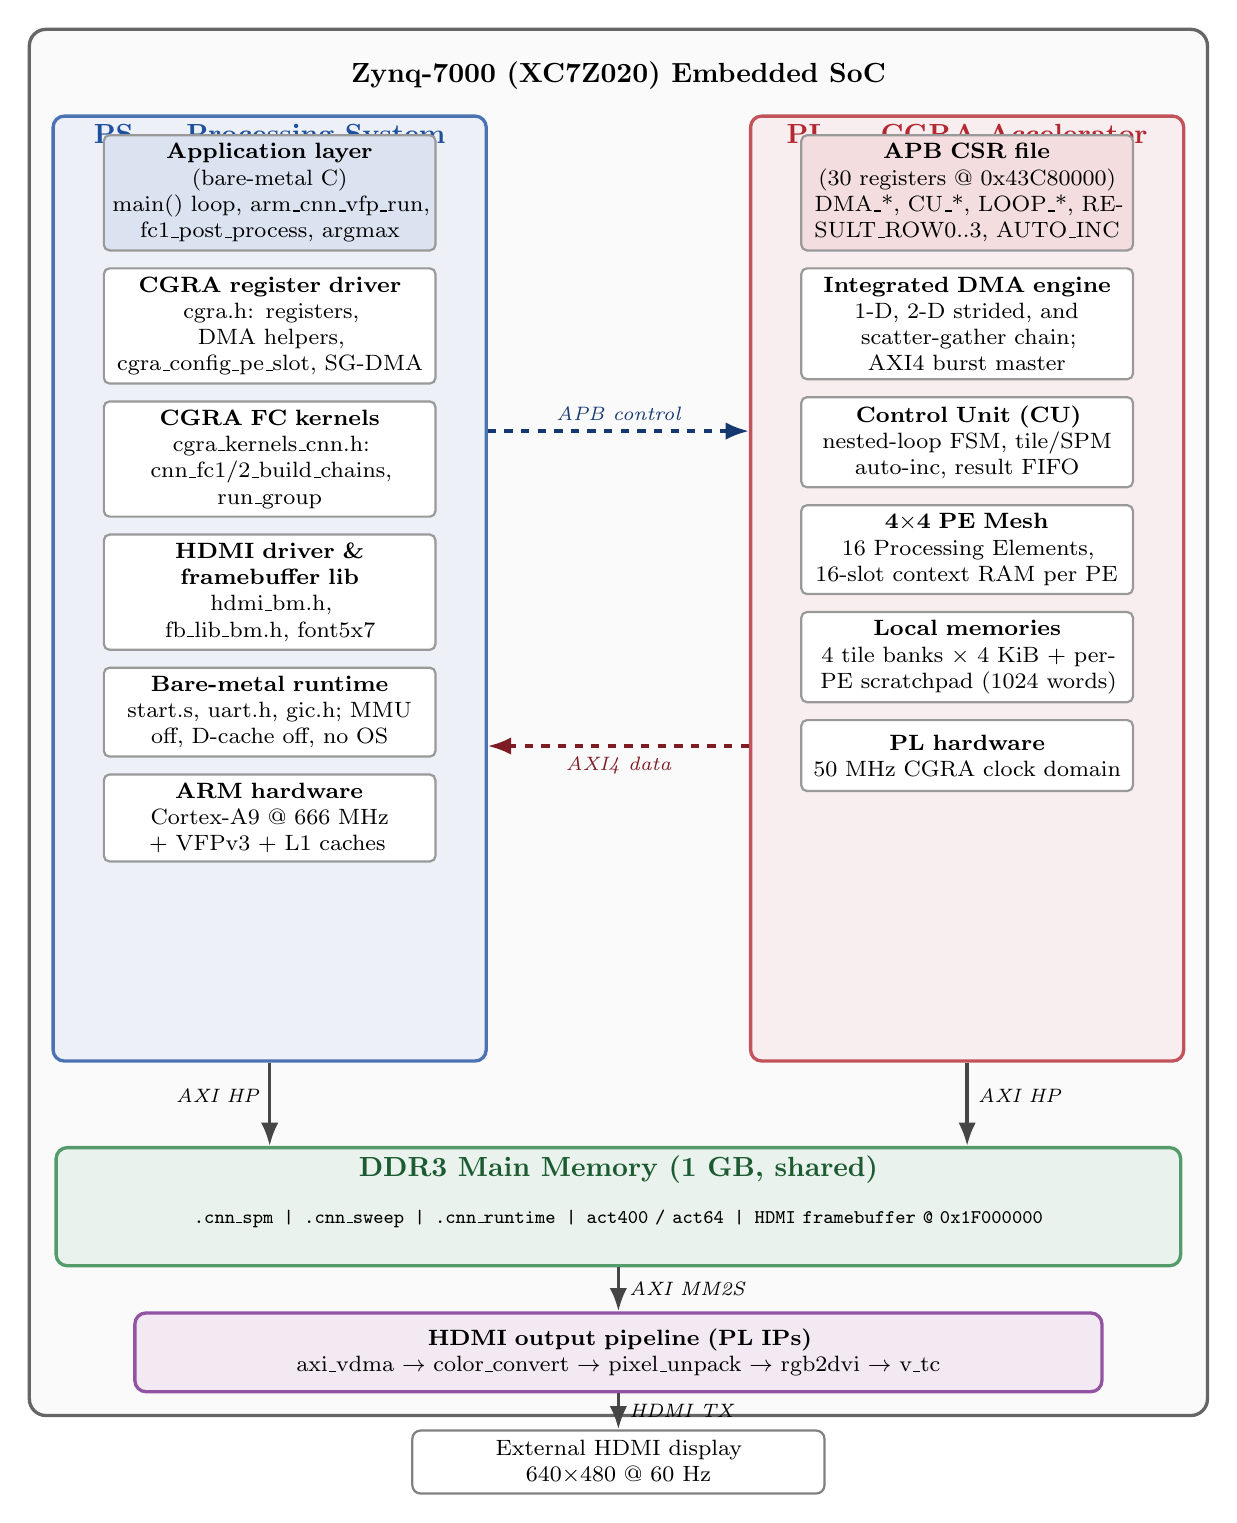
\begin{tikzpicture}[
    node distance = 2.5cm and 3cm,
    every node/.append style = {font=\footnotesize},
    soc/.style    = {rectangle, draw=black!60, fill=gray!4, very thick,
                     rounded corners=6pt, inner sep=8pt},
    psbox/.style  = {rectangle, draw=armblue!80, fill=armblue!8,
                     very thick, rounded corners=4pt, align=center,
                     minimum width=5.5cm, minimum height=12cm,
                     inner sep=4pt},
    plbox/.style  = {rectangle, draw=cgrared!80, fill=cgrared!8,
                     very thick, rounded corners=4pt, align=center,
                     minimum width=5.5cm, minimum height=12cm,
                     inner sep=4pt},
    ddrbox/.style = {rectangle, draw=ddrgreen!80, fill=ddrgreen!10,
                     very thick, rounded corners=4pt, align=center,
                     text width=14cm, minimum height=1.5cm,
                     inner sep=4pt},
    hdmibx/.style = {rectangle, draw=hdmipurple!80, fill=hdmipurple!10,
                     very thick, rounded corners=4pt, align=center,
                     text width=12cm, minimum height=1cm,
                     inner sep=4pt},
    extbx/.style  = {rectangle, draw=black!50, fill=white, thick,
                     rounded corners=3pt, align=center,
                     text width=5cm, minimum height=0.8cm},
    %% KEY FIX (user request 2): every inner block has text width=4cm so
    %% long sentences wrap into multiple lines instead of pushing the
    %% block width outward and colliding with the neighbouring lane.
    inner/.style  = {rectangle, draw=black!40, fill=white, thick,
                     rounded corners=2pt, align=center,
                     text width=4cm, inner sep=3pt,
                     minimum height=0.9cm, font=\footnotesize},
    blocktitle/.style = {font=\bfseries, anchor=north},
    busArr/.style = {-Latex, very thick, draw=gray!55!black},
    apbArr/.style = {-Latex, very thick, draw=armblue!70!black, dashed},
    dmaArr/.style = {-Latex, very thick, draw=cgrared!70!black, dashed},
    labelArr/.style = {font=\scriptsize\itshape}
]

% ===== Title bar =====
\node[font=\bfseries] (title) at (0, 7.2)
   {Zynq-7000 (XC7Z020) Embedded SoC};

% ===== PS side (left) =====
\node[psbox, anchor=north west] (ps) at (-7.2, 6.7) {};
\node[blocktitle] at (ps.north)
   {\textcolor{armblue}{PS --- Processing System}};

\node[inner, fill=armblue!16, below=2.5mm of ps.north] (app)
   {\textbf{Application layer} \\ (bare-metal C) \\
    main() loop, arm\_cnn\_vfp\_run, fc1\_post\_process, argmax};
\node[inner, below=2mm of app] (drvA)
   {\textbf{CGRA register driver} \\
    cgra.h: registers, DMA helpers, cgra\_config\_pe\_slot, SG-DMA};
\node[inner, below=2mm of drvA] (drvB)
   {\textbf{CGRA FC kernels} \\
    cgra\_kernels\_cnn.h: cnn\_fc1/2\_build\_chains, run\_group};
\node[inner, below=2mm of drvB] (drvC)
   {\textbf{HDMI driver \& framebuffer lib} \\
    hdmi\_bm.h, fb\_lib\_bm.h, font5x7};
\node[inner, below=2mm of drvC] (rt)
   {\textbf{Bare-metal runtime} \\
    start.s, uart.h, gic.h; MMU off, D-cache off, no OS};
\node[inner, below=2mm of rt] (hw)
   {\textbf{ARM hardware} \\
    Cortex-A9 @ 666 MHz + VFPv3 + L1 caches};

% ===== PL side (right) =====
\node[plbox, anchor=north east] (pl) at (7.2, 6.7) {};
\node[blocktitle] at (pl.north)
   {\textcolor{cgrared}{PL --- CGRA Accelerator}};

\node[inner, fill=cgrared!16, below=2.5mm of pl.north] (csr)
   {\textbf{APB CSR file} \\ (30 registers @ 0x43C80000) \\
    DMA\_*, CU\_*, LOOP\_*, RESULT\_ROW0..3, AUTO\_INC};
\node[inner, below=2mm of csr] (dma)
   {\textbf{Integrated DMA engine} \\
    1-D, 2-D strided, and scatter-gather chain; AXI4 burst master};
\node[inner, below=2mm of dma] (cu)
   {\textbf{Control Unit (CU)} \\
    nested-loop FSM, tile/SPM auto-inc, result FIFO};
\node[inner, below=2mm of cu] (mesh)
   {\textbf{4$\times$4 PE Mesh} \\
    16 Processing Elements, 16-slot context RAM per PE};
\node[inner, below=2mm of mesh] (mem)
   {\textbf{Local memories} \\
    4 tile banks $\times$ 4 KiB + per-PE scratchpad (1024 words)};
\node[inner, below=2mm of mem] (clk)
   {\textbf{PL hardware} \\
    50 MHz CGRA clock domain};

% ===== Bus arrows between PS and PL =====
\coordinate (ap1) at ($(ps.east)+(0,2.0)$);
\coordinate (ap2) at ($(pl.west)+(0,2.0)$);
\coordinate (dm1) at ($(pl.west)+(0,-2.0)$);
\coordinate (dm2) at ($(ps.east)+(0,-2.0)$);

\draw[apbArr] (ap1) -- (ap2)
   node[midway, above, labelArr, text=armblue!70!black]{APB control};
\draw[dmaArr] (dm1) -- (dm2)
   node[midway, below, labelArr, text=cgrared!70!black]{AXI4 data};

% ===== DDR =====
\node[ddrbox, anchor=north] (ddr) at (0, -6.4) {};
\node[blocktitle, anchor=north] at (ddr.north)
   {\textcolor{ddrgreen!70!black}{DDR3 Main Memory (1 GB, shared)}};
\node[anchor=center, font=\scriptsize\ttfamily, align=center,
      text width=13cm] at ($(ddr.center)+(0,-0.15)$) {
   .cnn\_spm \,|\, .cnn\_sweep \,|\, .cnn\_runtime \,|\,
   act400 / act64 \,|\, HDMI framebuffer @ 0x1F000000
};

% Vertical buses PS <-> DDR and PL <-> DDR
\draw[busArr] (ps.south) -- ($(ps.south |- ddr.north)$)
   node[pos=0.4, left, labelArr] {AXI HP};
\draw[busArr] (pl.south) -- ($(pl.south |- ddr.north)$)
   node[pos=0.4, right, labelArr] {AXI HP};

% ===== HDMI pipeline =====
\node[hdmibx, anchor=north] (hdmiip) at (0, -8.5) {%
   \textbf{HDMI output pipeline (PL IPs)} \\
   axi\_vdma $\to$ color\_convert $\to$ pixel\_unpack $\to$
   rgb2dvi $\to$ v\_tc};
\draw[busArr] (ddr.south) -- (hdmiip.north)
   node[midway, right, labelArr] {AXI MM2S};

% ===== External display =====
\node[extbx, anchor=north] (display) at (0, -10.0)
   {External HDMI display \\ 640$\times$480 @ 60 Hz};
\draw[busArr] (hdmiip.south) -- (display.north)
   node[midway, right, labelArr] {HDMI TX};

% ===== Outer SoC chassis =====
\begin{pgfonlayer}{background}
\node[soc, fit=(title)(ps)(pl)(ddr)(hdmiip)] (socbox) {};
\end{pgfonlayer}

\end{tikzpicture}%
}
\caption{System software architecture and ARM--CGRA interaction.
The blue (PS) and red (PL) blocks are physical halves of the Zynq SoC.
Inside the PS block, sub-blocks are layered from the application code
(top) down to the bare-metal runtime and the underlying ARM hardware.
Inside the PL block, the CGRA's externally-visible interfaces (APB CSR
and DMA) are at the top, with the compute fabric beneath. Dashed arrows
between PS and PL are the two logical interfaces: APB carries narrow
control words; AXI4 carries wide bulk data. Both halves share the DDR3
memory below them; the HDMI output pipeline draws its framebuffer from
the same DDR.}
\label{fig:arch}
\end{figure}

\paragraph{Three layers on the PS side.}
The host stack is a strict three-layer cake. The \emph{bare-metal
runtime} at the bottom --- the reset vector in \file{start.s}, the GIC
driver in \file{gic.{h,c}}, and the polled UART driver in
\file{uart.h} --- runs with the Memory Management Unit disabled, the
L1 data cache off, and no operating system whatsoever; it provides
exactly enough scaffolding for C code to execute from on-chip memory
and for hardware peripherals to be reachable at their physical
addresses. Above this, a thin \emph{driver / hardware-abstraction
layer} exposes the CGRA's register-level operations as inline C
functions (\file{cgra.h}), the silicon-validated FC kernel chains as
higher-level routines (\file{cgra\_kernels\_cnn.h}), and the HDMI
framebuffer and rendering primitives (\file{hdmi\_bm.h},
\file{fb\_lib\_bm.h}). At the top, the \emph{application layer} --- the
demo's \code{main()}, the VFP convolution reference, the FC
post-processing, and the argmax classifier --- combines those
abstractions into the per-frame inference loop. This layering keeps
the application code free of any direct register pokes and keeps the
register-level code free of any application-specific concepts.

\paragraph{The CGRA's two external interfaces.}
Seen from the host, the CGRA exposes exactly two interfaces. The
\emph{APB control-status interface} (Advanced Peripheral Bus, 32~bits,
serialized) is a narrow channel used by the host to write configuration
words to the CGRA's 30 registers and read back status flags. Every
operation the host initiates --- start a DMA, start the CU, change the
hardware-loop count, drain the result registers --- is one or more APB
writes or reads. The \emph{AXI4 master interface} (Advanced eXtensible
Interface, 64-bit data, burst-capable) is the wide data channel by
which the CGRA's integrated DMA engine reads operands from DDR and
writes them into the tile memory, the per-PE scratchpad, or the PE
configuration RAM, and through which it can also write results back
to DDR. The APB channel touches single 32-bit words and operates in
the tens-of-nanoseconds-per-write regime; the AXI4 channel moves
4096-byte tile banks in single-digit microseconds. Keeping these
roles strictly separated --- never trying to stream bulk data through
APB --- is the discipline behind the demo's sub-millisecond FC
timings.

\paragraph{Shared DDR as the data exchange.}
Both the ARM core (through its native AXI bus into the PS DDR
controller) and the CGRA's DMA engine (through an AXI High-Performance
slave port on the PS) reach the same physical DDR3. All bulk data
exchanged between the two --- the test images in \code{.cnn\_sweep},
the FC weight blob in \code{.cnn\_spm}, the inter-layer activations
\code{act400} and \code{act64}, and the HDMI framebuffer at
\addr{1F000000} --- lives in DDR. The CGRA never reads or writes
on-chip memory; the ARM never reads or writes the CGRA's internal
tile memory or scratchpads (those are reachable only as DMA
destinations). The DDR is therefore both the message-passing fabric
between the two compute domains and the staging area for the HDMI
output pipeline that consumes the framebuffer at scan-out time. This
``everything goes through DDR'' discipline means that the only
synchronization primitive the host needs is a properly-ordered
\code{dsb} barrier before kicking the CGRA, ensuring that the
activation writes it just performed have actually drained out of the
ARM write-buffer into DDR before the CGRA's DMA tries to read them.

\paragraph{HDMI as a passive consumer.}
The HDMI output pipeline (\code{axi\_vdma}, \code{color\_convert},
\code{pixel\_unpack}, \code{rgb2dvi}, \code{v\_tc}) runs continuously
in PL and is a passive consumer of the DDR framebuffer. Once the host
has configured these IPs at boot through their APB-mapped registers,
they require no per-frame ARM intervention --- the VDMA simply
re-reads the same 921{,}600-byte region of DDR 60 times per second
and pushes the resulting pixel stream out the HDMI TX pins. The
application's role per frame reduces to overwriting the framebuffer's
contents with new pixels through volatile pointer writes; no
notification to the HDMI pipeline is required, only the same
\code{dsb} barrier that guarantees the writes have reached DDR before
the next VDMA scan begins.

\subsection{Architectural Partitioning}
\label{ssec:partitioning}

The software architecture observes a strict separation between
\textbf{host-side concerns} (executed on the Cortex-A9) and
\textbf{accelerator-side concerns} (executed on the CGRA fabric).
\Cref{tab:partitioning} enumerates the per-stage assignment.

\begin{table}[!htbp]
\centering
\caption{Partitioning of software concerns between the ARM core and the
CGRA fabric. The ``Executor'' column gives the hardware target; the
implementing source file is named in the ``Rationale'' column where it
adds context.}
\label{tab:partitioning}
\footnotesize
\setlength{\tabcolsep}{6pt}
\begin{tabularx}{\textwidth}{@{}>{\raggedright\arraybackslash}X >{\centering\arraybackslash}p{1.6cm} >{\raggedright\arraybackslash}X@{}}
\toprule
\textbf{Concern} & \textbf{Executor} & \textbf{Rationale} \\
\midrule
Boot, SLCR clock setup, VFP enable, BSS zero & ARM &
Required before any application code can run (\file{start.s}). \\[2pt]
HDMI bring-up: dynclk MMCM, VTC, VDMA, color-convert, pixel-unpack & ARM &
Sequential register-write protocol; no acceleration benefit
(\file{hdmi\_bm.c}). \\[2pt]
Conv1+ReLU+Pool1+Conv2+ReLU+Pool2 & ARM-VFP &
The CGRA's per-pixel Conv kernel saturates its INT32 result FIFO on a
9-MAC $\times$ 8-channel sum; scalar VFP avoids this and yields the
ground-truth float reference (\file{arm\_cnn\_bm.c}). \\[2pt]
Flatten + per-image quantization (HWC$\rightarrow$CHW, max-abs to INT16) &
ARM-VFP &
Negligible compute; produces the \code{act400[400]} vector consumed
by all three FC paths. \\[2pt]
\textbf{FC1 ($400{\times}64$) and FC2 ($64{\times}10$) dense matmul} &
\textbf{CGRA} &
The SPM\_AUTO\_INC + TILE\_AUTO\_INC + 4-row-parallel pattern is the
kernel the CGRA is optimized for (\file{cgra\_kernels\_cnn.h}). \\[2pt]
Bias add, ReLU, requantize between FC1 and FC2 & ARM &
64 scalar operations; faster than configuring a CGRA bypass kernel. \\[2pt]
Argmax over 10 FC2 logits & ARM & 10-element reduction; trivial. \\[2pt]
Cycle-counter timing (PMCCNTR) & ARM &
Required for the head-to-head comparison. \\[2pt]
Framebuffer rendering: rectangles, glyphs, image blit & ARM &
Volatile writes into the HDMI framebuffer at \addr{1F000000}
(\file{fb\_lib\_bm.c}). \\
\bottomrule
\end{tabularx}
\end{table}

The CGRA is invoked only for the workload pattern in which it dominates
the ARM core --- dense matrix multiplication with regular weight reuse
--- leaving all serial, irregular, or trivially-small operations on
the host side. This partitioning is the source of the measured
3.74$\times$ speedup on the FC stage and of the demo's 97\% end-to-end
classification accuracy.

\subsection{Per-Frame Execution Flowchart}
\label{ssec:flowchart}

Where Figure~\ref{fig:arch} answers ``what is connected to what,''
Figure~\ref{fig:swimlane} answers ``what happens when'' --- a swim-lane
diagram of the actual control flow executed by the demo ELF on every
inference frame. The left column captures ARM-side operations; the
right column captures CGRA-side operations; dashed green arrows
indicate ARM$\leftrightarrow$CGRA handoffs that cross the boundary
introduced in the previous subsection (APB control writes or
DDR-resident SG-DMA descriptor chains). The blocks are numbered 1--13
so the step-by-step description that follows the figure can reference
each one directly.

\begin{figure}[!htbp]
\centering
\resizebox{0.96\textwidth}{!}{%
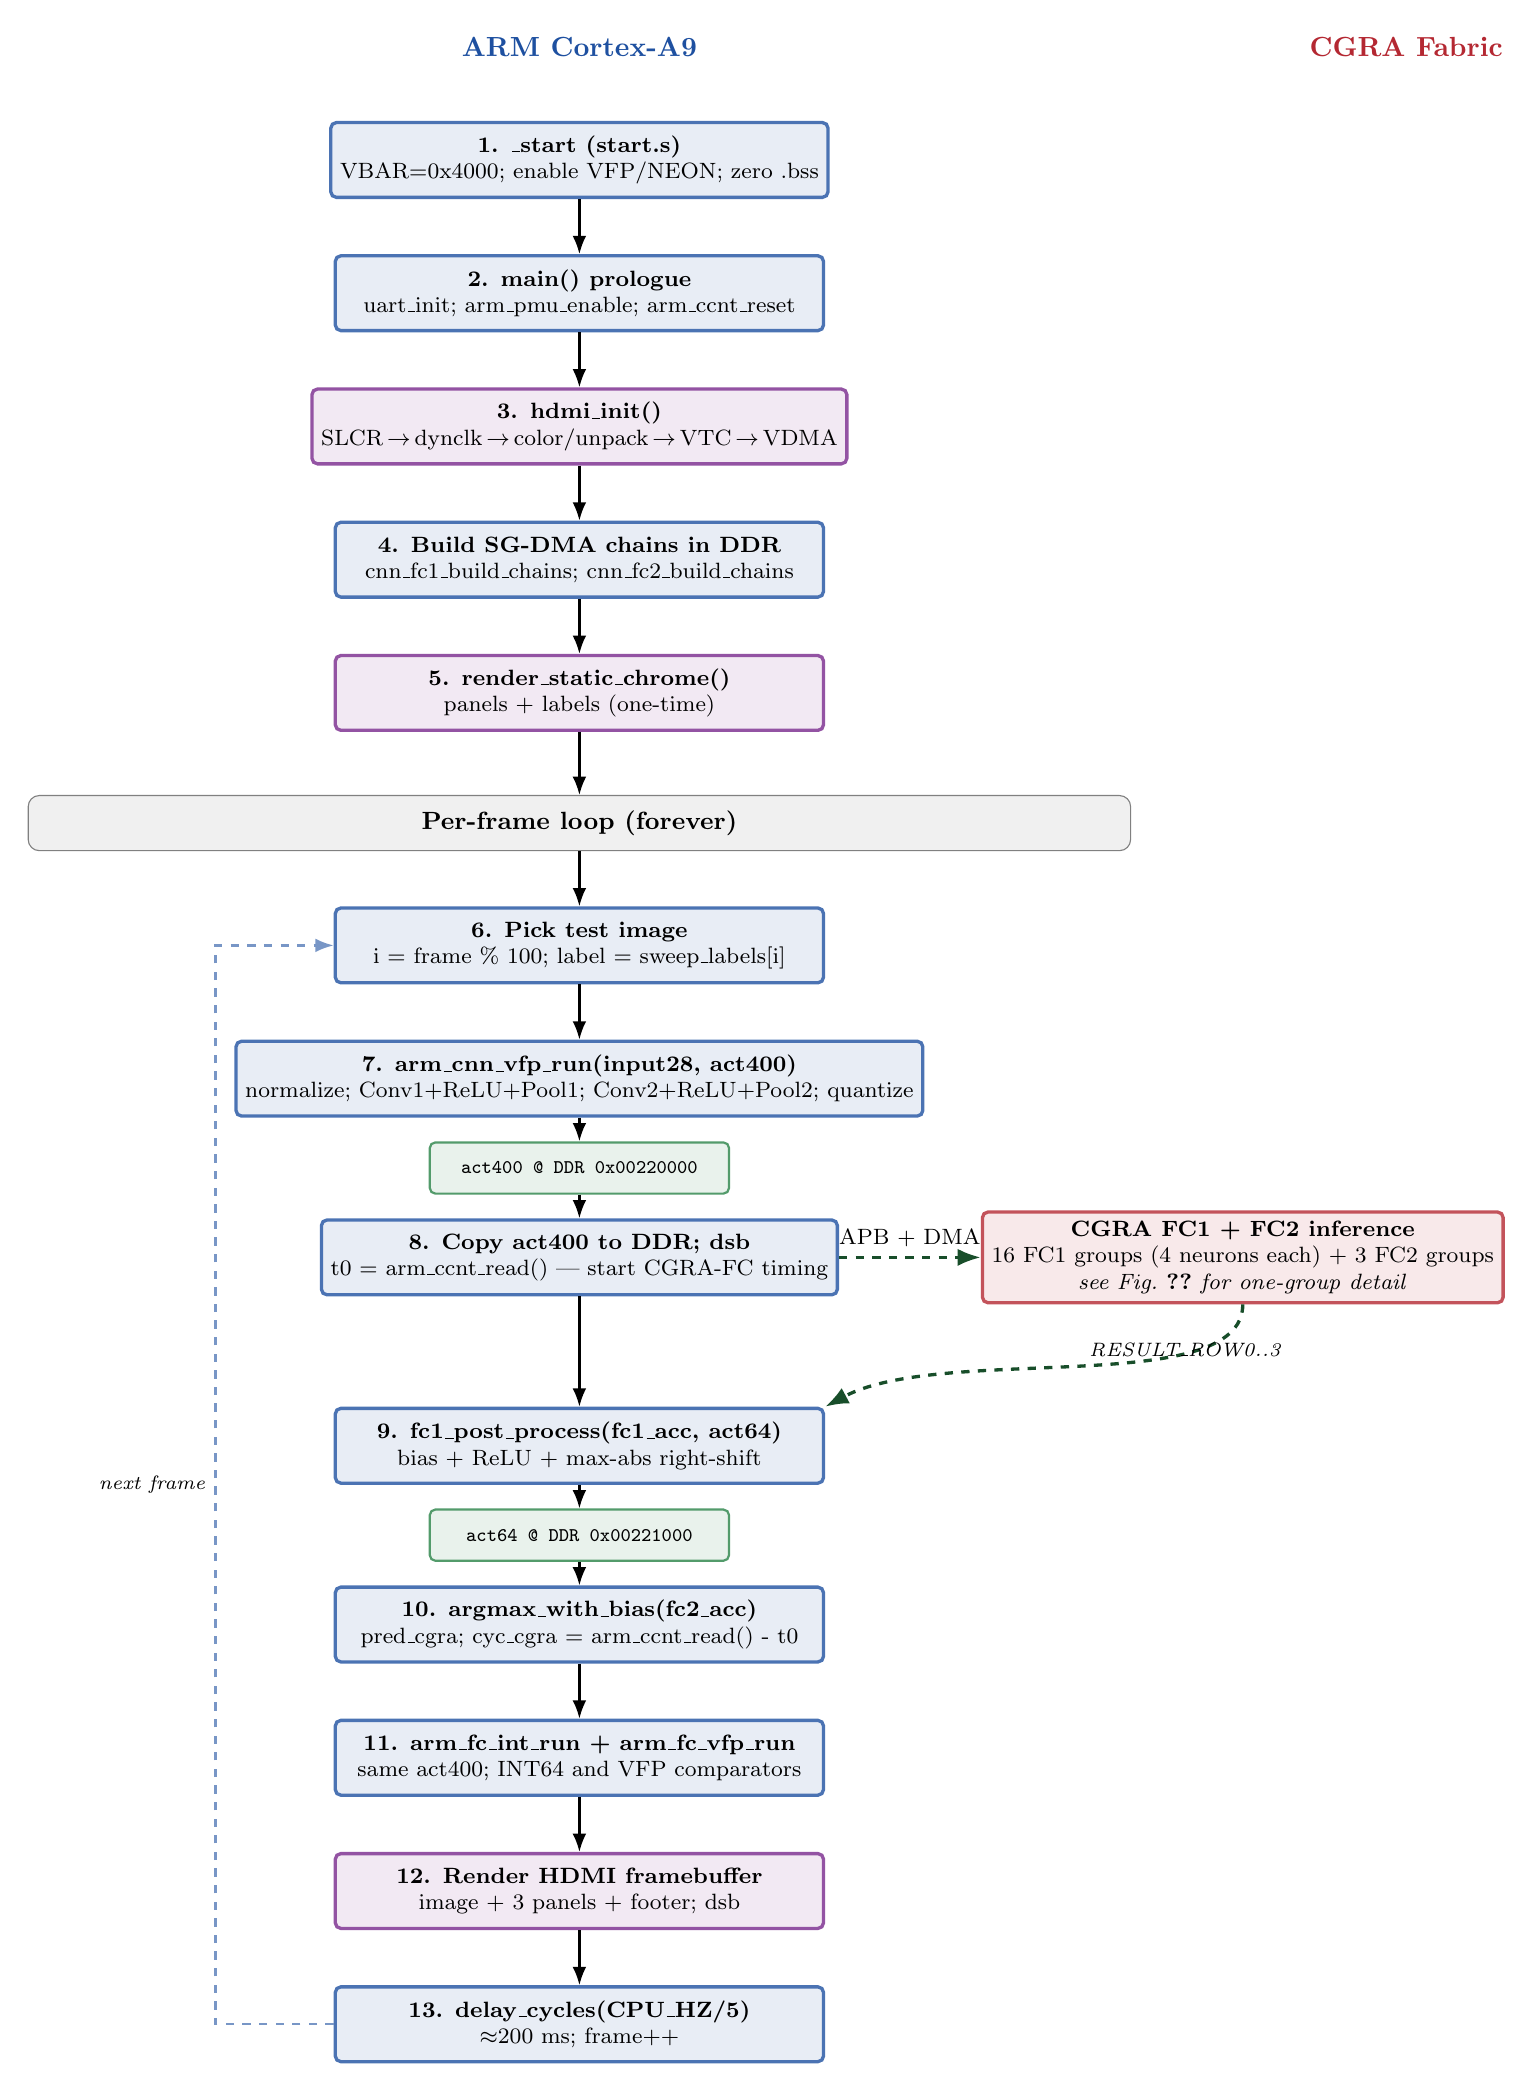
\begin{tikzpicture}[
    node distance = 7mm and 18mm,
    every node/.append style = {font=\footnotesize},
    armnode/.style  = {rectangle, draw=armblue!80, fill=armblue!10,
                       very thick, minimum width=6.2cm, minimum height=0.95cm,
                       align=center, rounded corners=2pt},
    cgranode/.style = {rectangle, draw=cgrared!80, fill=cgrared!10,
                       very thick, minimum width=6.2cm, minimum height=0.95cm,
                       align=center, rounded corners=2pt},
    hdminode/.style = {rectangle, draw=hdmipurple!80, fill=hdmipurple!10,
                       very thick, minimum width=6.2cm, minimum height=0.95cm,
                       align=center, rounded corners=2pt},
    ddrbox/.style   = {rectangle, draw=ddrgreen!80, fill=ddrgreen!10,
                       thick, minimum width=3.8cm, minimum height=0.65cm,
                       align=center, font=\scriptsize\ttfamily,
                       rounded corners=2pt},
    arrow/.style    = {-Latex, thick},
    handoff/.style  = {-Latex, very thick, dashed, draw=ddrgreen!60!black,
                       font=\scriptsize\itshape},
    looplbl/.style  = {rectangle, draw=black!50, fill=gray!12,
                       rounded corners=4pt, minimum width=14cm,
                       minimum height=0.7cm, font=\bfseries\small,
                       align=center}
]

% --- Lane titles ---
\node (armT)  at (0,0) [font=\bfseries] {\textcolor{armblue}{ARM Cortex-A9}};
\node (cgraT) at (10.5,0) [font=\bfseries] {\textcolor{cgrared}{CGRA Fabric}};

% --- Boot chain (ARM only) ---
\node[armnode, below=of armT]      (boot)     {\textbf{1. \_start (start.s)}\\
   VBAR=0x4000; enable VFP/NEON; zero .bss};
\node[armnode, below=of boot]      (prologue) {\textbf{2. main() prologue}\\
   uart\_init; arm\_pmu\_enable; arm\_ccnt\_reset};
\node[hdminode, below=of prologue] (hdmi)     {\textbf{3. hdmi\_init()}\\
   SLCR\,$\to$\,dynclk\,$\to$\,color/unpack\,$\to$\,VTC\,$\to$\,VDMA};
\node[armnode, below=of hdmi]      (chains)   {\textbf{4. Build SG-DMA chains in DDR}\\
   cnn\_fc1\_build\_chains; cnn\_fc2\_build\_chains};
\node[hdminode, below=of chains]   (chrome)   {\textbf{5. render\_static\_chrome()}\\
   panels + labels (one-time)};

% --- Loop header ---
\node[looplbl, below=8mm of chrome] (loop) {Per-frame loop (forever)};

% --- Per-frame chain (ARM) ---
\node[armnode, below=of loop]      (pick) {\textbf{6. Pick test image}\\
   i = frame \% 100; label = sweep\_labels[i]};
\node[armnode, below=of pick]      (vfp)  {\textbf{7. arm\_cnn\_vfp\_run(input28, act400)}\\
   normalize; Conv1+ReLU+Pool1; Conv2+ReLU+Pool2; quantize};
\node[ddrbox,  below=3mm of vfp]   (ddrA) {act400 @ DDR \texttt{0x00220000}};
\node[armnode, below=3mm of ddrA]  (kick) {\textbf{8. Copy act400 to DDR; dsb}\\
   t0 = arm\_ccnt\_read() --- start CGRA-FC timing};

% --- CGRA inset block (aligned to the right of the kick stage) ---
\node[cgranode, right=of kick] (cgrafc) {\textbf{CGRA FC1 + FC2 inference}\\
   16 FC1 groups (4 neurons each) + 3 FC2 groups\\
   \emph{see Fig.~\ref{fig:fc-group} for one-group detail}};

% --- Continuation on ARM ---
\node[armnode, below=14mm of kick]  (post)   {\textbf{9. fc1\_post\_process(fc1\_acc, act64)}\\
   bias + ReLU + max-abs right-shift};
\node[ddrbox,  below=3mm of post]   (ddrB)   {act64 @ DDR \texttt{0x00221000}};
\node[armnode, below=3mm of ddrB]   (argmax) {\textbf{10. argmax\_with\_bias(fc2\_acc)}\\
   pred\_cgra; cyc\_cgra = arm\_ccnt\_read() - t0};
\node[armnode, below=of argmax]     (others) {\textbf{11. arm\_fc\_int\_run + arm\_fc\_vfp\_run}\\
   same act400; INT64 and VFP comparators};
\node[hdminode, below=of others]    (render) {\textbf{12. Render HDMI framebuffer}\\
   image + 3 panels + footer; dsb};
\node[armnode, below=of render]     (delay)  {\textbf{13. delay\_cycles(CPU\_HZ/5)}\\
   $\approx$200 ms; frame++};

% --- Vertical flow arrows along the ARM column ---
\foreach \src/\dst in
   {boot/prologue, prologue/hdmi, hdmi/chains, chains/chrome,
    chrome/loop, loop/pick, pick/vfp, vfp/ddrA, ddrA/kick,
    kick/post, post/ddrB, ddrB/argmax, argmax/others,
    others/render, render/delay}
   \draw[arrow] (\src) -- (\dst);

% --- ARM <-> CGRA handoffs (only at well-defined boundaries) ---
\draw[handoff] (kick.east) -- node[above,sloped]{APB + DMA} (cgrafc.west);
\draw[handoff] (cgrafc.south) .. controls +(0,-12mm) and +(15mm,8mm) ..
   node[above right, font=\scriptsize\itshape]{RESULT\_ROW0..3} (post.north east);

% --- Loopback arrow on the left side ---
\draw[arrow, dashed, draw=armblue!60]
   (delay.west) -- ++(-15mm,0)
   |- node[pos=0.25, left, font=\scriptsize\itshape]{next frame} (pick.west);

\end{tikzpicture}%
}
\caption{Per-frame execution flow. Boot stages (top, above the labelled
bar) execute once; per-frame stages execute indefinitely. Blue
boxes are ARM-side, red boxes are CGRA-side, purple boxes are
HDMI-pipeline operations, and green mini-boxes mark DDR-resident handoff
buffers. Dashed green arrows are APB/DMA crossings of the ARM--CGRA
boundary. The CGRA-FC block expands to Fig.~\ref{fig:fc-group}.}
\label{fig:swimlane}
\end{figure}

The flowchart is hierarchical: the per-frame loop executes
indefinitely, while the boot stages run once. The CGRA is invoked
\emph{twice} per frame (FC1 and FC2), with the ARM core orchestrating
data movement and post-processing in between. The remainder of this
subsection walks through every numbered block; Figure~\ref{fig:fc-group}
then zooms into the internal six-step structure of one
\code{cnn\_fc\_run\_group()} call.

\paragraph{Boot phase (steps 1--5, executed once at power-on).}
\begin{enumerate}[leftmargin=2.1em, label=\textbf{Step \arabic*.},
                  itemsep=4pt, topsep=2pt]
\item \textbf{Reset vector in \file{start.s}.} On power-on the
Cortex-A9 starts execution at the reset vector. The hand-written
assembly sets the Vector Base Address Register (VBAR) to
\addr{00004000}, enables the VFP/NEON coprocessor (CPACR bits cp10
and cp11) and clears FPEXC, zeros the \code{.bss} section in OCM,
and finally jumps to the C \code{main()}. The MMU and the L1 data
cache are deliberately left disabled --- all subsequent memory
accesses are physical and uncached, which keeps the cycle-counter
measurements deterministic.

\item \textbf{\code{main()} prologue.} The first few statements of
\code{main()} bring up the host's instrumentation infrastructure.
\code{uart\_init()} configures the Zynq PS UART0 for 115200 baud, 8N1,
on MIO\,14/15. \code{arm\_pmu\_enable()} writes the Performance
Monitor Control Register (PMCR) to enable the on-chip cycle counter,
and \code{arm\_ccnt\_reset()} clears it so that all subsequent
\code{arm\_ccnt\_read()} calls return a monotonically-increasing
cycle count. Without these calls, the head-to-head FC timings would
be impossible.

\item \textbf{HDMI pipeline bring-up.} \code{hdmi\_init()} brings up
the five PL IPs that make up the video output. It first unlocks the
PS SLCR registers, sets FCLK0 to 100 MHz (the reference clock that
\code{axi\_dynclk} expects), re-locks SLCR, and then calls
\code{hdmi\_force\_idle()} to quench any leftover state from a prior
ELF run. It then programs the MMCM inside \code{axi\_dynclk} to
synthesize a 25.175 MHz pixel clock, loads an identity 3$\times$3
colour-matrix into \code{color\_convert}, sets \code{pixel\_unpack}
to the V\_24 (3-byte BGR) mode, programs \code{v\_tc} for 640$\times$480
@ 60 Hz timing, and finally arms \code{axi\_vdma} in MM2S mode
pointing at the framebuffer at \addr{1F000000}.

\item \textbf{Build SG-DMA descriptor chains in DDR.} The host now
calls \code{cnn\_fc1\_build\_chains()} followed by
\code{cnn\_fc2\_build\_chains()}. These two routines populate a
region of DDR with linked lists of \code{cgra\_sg\_dma\_descriptor\_t}
records --- one chain per phase of an FC group (SPM-preload, ACC\_CLR,
MAC-restore, east-readout, plus a one-time east-chain init). After
this step, dispatching a 64-neuron FC1 layer or a 10-neuron FC2
layer requires no further descriptor construction at run time; the
host simply writes a chain's head pointer into the
\reg{DMA\_DESC\_HEAD} register and asserts the chain-start bit.

\item \textbf{Render static chrome.} Finally, \code{render\_static\_chrome()}
paints the panel rectangles, the labels (``CGRA-FC'', ``ARM-INT-FC'',
``ARM-VFP-FC''), and the screen titles to the HDMI framebuffer. These
elements never change across frames, so they are written once at boot
rather than on each per-frame render pass. A single \code{dsb}
guarantees the writes have reached DDR before the VDMA's next scan-out
cycle picks them up.
\end{enumerate}

\paragraph{Per-frame phase (steps 6--13, repeated forever).}
\begin{enumerate}[leftmargin=2.1em, label=\textbf{Step \arabic*.}, start=6,
                  itemsep=4pt, topsep=2pt]
\item \textbf{Pick the next test image.} The host computes
\code{i = frame \% SWEEP\_N\_IMAGES} to index into the 100-image
fixture and looks up \code{label = sweep\_labels[i]} for accuracy
bookkeeping. Both arrays live in the read-only \code{.cnn\_sweep}
DDR section, so no copy is needed --- the ARM operates on
pointers directly into the fixture.

\item \textbf{ARM-VFP convolutional front-end.} The function
\code{arm\_cnn\_vfp\_run()} takes the raw \code{sweep\_input28[i]}
array as input and fills the output buffer \code{act400[400]} after
running the full floating-point convolutional pipeline on the ARM
core. Inside it,
\code{normalize\_input()} converts each \code{uint8\_t} pixel into a
VFPv3 float and applies the MNIST whitening transform; Conv1
(3$\times$3, 1$\to$8 channels) is computed in place; \code{relu\_inplace()}
clamps negatives to zero; \code{maxpool\_2x2()} reduces to 13$\times$13$\times$8;
the same Conv$+$ReLU$+$Pool sequence is repeated for Conv2 (3$\times$3,
8$\to$16); the 5$\times$5$\times$16 tensor is transposed from HWC to CHW order
to match PyTorch's flatten convention; and finally
\code{quantize\_to\_int32()} computes the per-image max-abs and
rescales the 400 values to the INT16 dynamic range required by FC1.
The output, \code{act400[400]}, is a stack-resident INT32 buffer.

\item \textbf{Stage the activation in DDR and start timing.} The host
copies \code{act400[400]} into the DDR-resident staging buffer at
\reg{ACT400\_DDR\,=\,0x00220000} using a simple C loop of volatile
INT32 writes. A \code{dsb} memory barrier flushes the ARM
write-buffer; without it, the CGRA's DMA engine could begin reading
DDR before the ARM's writes have actually landed. Then
\code{t0\,=\,arm\_ccnt\_read()} captures the starting cycle so the
CGRA-FC stage can be timed independently of the Conv stage above.

\item \textbf{CGRA executes FC1 and FC2.} This is the principal
ARM$\leftrightarrow$CGRA handoff. The host first calls
\code{cnn\_fc1\_tile\_preload(ACT400\_DDR)} which broadcasts the
1600-byte \code{act400} into all four CGRA tile banks via a single
1-D DMA transfer. It then iterates 16 times, once per output-neuron
group of four, calling \code{cnn\_fc1\_run\_group(g, \&fc1\_acc[g*4])}.
Each call triggers the six-step pre-built SG-DMA + CU sequence
detailed in Figure~\ref{fig:fc-group} (SPM preload, ACC\_CLR, MAC
restore, MAC CU run, east readout, APB drain) and produces four
INT32 dot products. The 64-element \code{fc1\_acc[]} array is then
post-processed (step~9), restaged in DDR, and the FC2 layer is
dispatched in the same way --- three groups instead of sixteen,
with the trailing two slots discarded since FC2 has only 10 outputs.

\item \textbf{FC1 post-processing on the ARM.} The 64 FC1 accumulator
values are passed to \code{fc1\_post\_process()}, which adds the
per-neuron bias from \code{mnist\_fc1\_bias\_q[]}, applies ReLU,
finds the maximum absolute value across all 64 outputs, and right-shifts
the entire buffer so that every value fits in INT16 range. The
shifted vector \code{act64[64]} is then staged in DDR at
\reg{ACT64\_DDR\,=\,0x00221000}, ready to feed FC2. This step
is too small (64 elements) to benefit from CGRA acceleration; the ARM
finishes it in well under one microsecond.

\item \textbf{Argmax and FC timing close.} After FC2 returns, the
host calls \code{argmax\_with\_bias(fc2\_acc)} which adds the
per-class bias from \code{mnist\_fc2\_bias\_q[]} to each of the ten
logits and returns the index of the maximum --- the predicted digit
class. \code{t1\,=\,arm\_ccnt\_read()} stops the timing window so
\code{cyc\_cgra\,=\,t1\,-\,t0} records exactly how many cycles the
FC stage consumed on the CGRA path.

\item \textbf{Re-time the same input on the two ARM-only comparators.}
The host now repeats the FC stage twice more, this time without the
CGRA: \code{arm\_fc\_int\_run(act400, cnn\_spm\_start)} executes the
same INT64-accumulator math entirely on the Cortex-A9 (matching the
CGRA's integer pipeline byte-for-byte), and
\code{arm\_fc\_vfp\_run(act400, cnn\_spm\_start)} executes the same
FC stage with VFPv3 floating-point MACs (the ``modern compiler
default'' comparator). Each run is wrapped in its own
\code{arm\_ccnt\_read()} window so the three timings are mutually
independent and directly comparable. All three paths see the same
input \code{act400}, so the only variable being measured is the FC
implementation itself.

\item \textbf{Render the result to HDMI.} \code{fbm\_draw\_image28()}
blits the raw 28$\times$28 input digit at 8$\times$ scale into a 224$\times$224
region of the framebuffer at the top of the screen.
\code{render\_panel()} then redraws each of the three result panels
with the latest \code{PRED}, \code{GT}, \code{$\mu$s}, and \code{FPS}
values; \code{render\_footer()} redraws the speedup ratios and the
three per-path accuracy counters. All of these primitives are simple
volatile writes into the DDR framebuffer; a final \code{dsb} ensures
the writes have drained before the VDMA's next scan-out pass.

\item \textbf{Inter-frame delay and loopback.}
\code{delay\_cycles(CPU\_HZ\,/\,5)} busy-waits for approximately
200 ms by polling the same PMU cycle counter used for the FC timing.
This dwell rate gives a defense audience roughly five frames per
second of visible inference, which is slow enough to read each
prediction comfortably and fast enough to convey live operation.
\code{frame++} and control returns to step~6 with the next image.
\end{enumerate}

\begin{figure}[!htbp]
\centering
\resizebox{0.92\textwidth}{!}{%
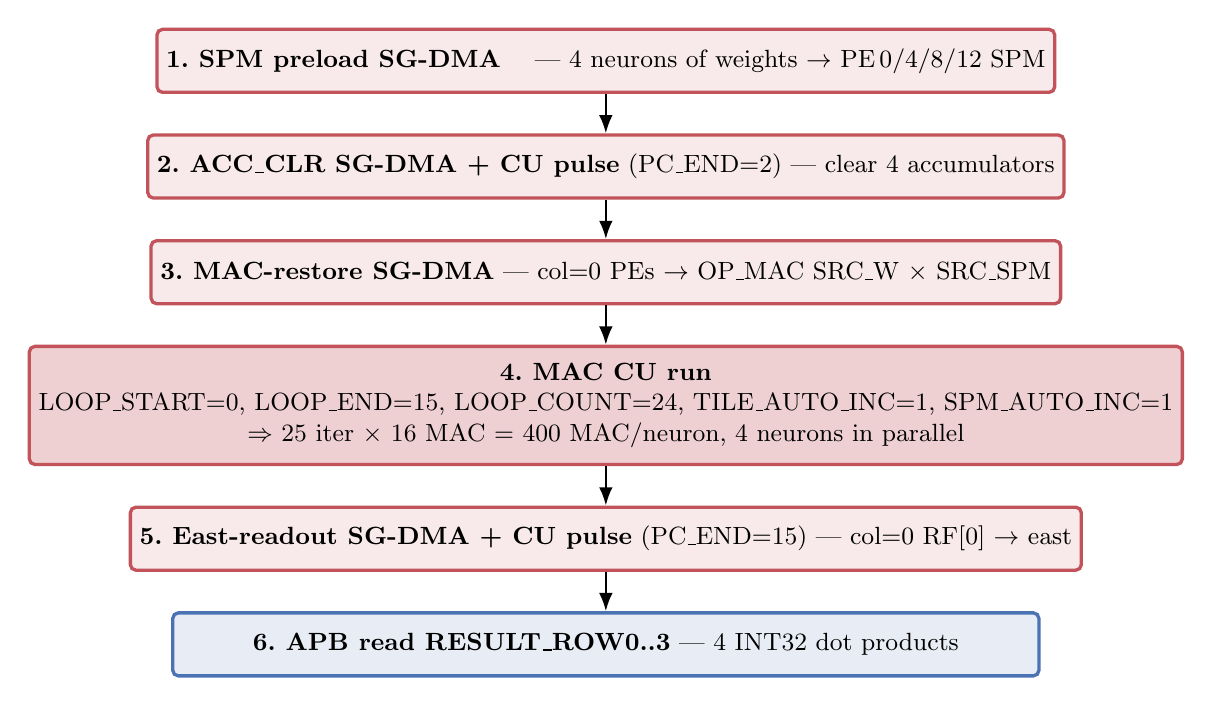
\begin{tikzpicture}[
   node distance = 5mm,
   every node/.append style = {font=\small},
   stepnode/.style = {rectangle, draw=cgrared!80, fill=cgrared!10,
                      very thick, minimum width=11cm, minimum height=0.8cm,
                      align=center, rounded corners=2pt},
   macstep/.style  = {rectangle, draw=cgrared!80, fill=cgrared!22,
                      very thick, minimum width=11cm, minimum height=1.5cm,
                      align=center, rounded corners=2pt},
   armstep/.style  = {rectangle, draw=armblue!80, fill=armblue!10,
                      very thick, minimum width=11cm, minimum height=0.8cm,
                      align=center, rounded corners=2pt},
   stepArrow/.style = {-Latex, thick}
]
\node[stepnode] (s1) {\textbf{1.\ SPM preload SG-DMA} \quad
   --- 4 neurons of weights $\to$ PE\,0/4/8/12 SPM};
\node[stepnode, below=of s1]  (s2)
   {\textbf{2.\ ACC\_CLR SG-DMA + CU pulse} (PC\_END=2) --- clear 4 accumulators};
\node[stepnode, below=of s2]  (s3)
   {\textbf{3.\ MAC-restore SG-DMA} --- col=0 PEs $\to$ OP\_MAC SRC\_W $\times$ SRC\_SPM};
\node[macstep,  below=of s3]  (s4)
   {\textbf{4.\ MAC CU run}\\
    LOOP\_START=0, LOOP\_END=15, LOOP\_COUNT=24,
    TILE\_AUTO\_INC=1, SPM\_AUTO\_INC=1\\
    $\Rightarrow$ 25 iter $\times$ 16 MAC = 400 MAC/neuron, 4 neurons in parallel};
\node[stepnode, below=of s4]  (s5)
   {\textbf{5.\ East-readout SG-DMA + CU pulse} (PC\_END=15) --- col=0 RF[0] $\to$ east};
\node[armstep,  below=of s5]  (s6)
   {\textbf{6.\ APB read RESULT\_ROW0..3} --- 4 INT32 dot products};
\foreach \a/\b in {s1/s2,s2/s3,s3/s4,s4/s5,s5/s6}
   \draw[stepArrow] (\a) -- (\b);
\end{tikzpicture}%
}
\caption{The six-step structure of one \code{cnn\_fc\_run\_group($g$)}
invocation. Steps 1--5 execute on the CGRA fabric without ARM
intervention; step 6 is the only APB read in the per-group critical
path. FC1 calls this 16 times per frame (64 outputs); FC2 calls it
3 times (10 outputs; last group has 2 valid neurons).}
\label{fig:fc-group}
\end{figure}

% =====================================================================
\section{Software Implementation}
\label{sec:ch4-impl}
% =====================================================================

\subsection{Initialization of Memory Regions}
\label{ssec:mmap}

In a Linux deployment the same address map would be accessed through
\code{mmap()} on \file{/dev/mem} or a UIO device node
(\code{open("/dev/uio0", O\_RDWR)} followed by
\code{mmap(..., PROT\_READ\,$|$\,PROT\_WRITE, MAP\_SHARED, fd, 0)}),
with the kernel translating between virtual and physical addresses.
In the present bare-metal deployment, however, the Cortex-A9 boots
with the MMU disabled and the L1 data cache off; all accesses are
physical and identity-mapped. Memory-mapped peripherals are accessed
by casting their physical addresses to \code{volatile uint32\_t *} and
dereferencing them directly. A single header, \file{cgra.h}, centralizes
the address constants and provides inline wrappers for register access
(\Cref{lst:cgra-h-base}).

\begin{lstlisting}[caption={Base addresses and register helpers for the
CGRA APB and DMA windows (excerpt from \file{cgra.h}).},
label={lst:cgra-h-base}]
#define CGRA_BASE          0x43C80000UL  /* APB base, PYNQ-base bolt-on */
#define CGRA_PFX_TILE      0x10000000UL  /* tile memory window         */
#define CGRA_PFX_CONFIG    0x20000000UL  /* per-PE config RAM window   */
#define CGRA_PFX_SPM       0x40000000UL  /* per-PE scratchpad window   */
#define CGRA_TILE_BCAST    (CGRA_PFX_TILE | 0x80000000UL)

static inline void cgra_wr(uint32_t off, uint32_t v) {
    *(volatile uint32_t *)(CGRA_BASE + off) = v;
}
static inline uint32_t cgra_rd(uint32_t off) {
    return *(volatile uint32_t *)(CGRA_BASE + off);
}
\end{lstlisting}

The CGRA's 30 APB control-status registers occupy offsets
\addr{00}--\addr{84} from \reg{CGRA\_BASE}; the application accesses
them exclusively through \code{cgra\_wr()}/\code{cgra\_rd()}. Three
additional address windows --- \reg{CGRA\_PFX\_TILE},
\reg{CGRA\_PFX\_CONFIG}, and \reg{CGRA\_PFX\_SPM} --- are \emph{not}
directly addressable from the ARM core. They are reachable only as
\emph{destinations} of the CGRA's integrated DMA engine; writing the
SPM, for instance, is accomplished by configuring the DMA with
\code{DMA\_DST = CGRA\_SPM\_PE\_ADDR(pe, 0)} and triggering a transfer.
This routing keeps the high-bandwidth weight and activation traffic
on the dedicated DMA path rather than serializing it through the
narrow APB bus.

The DDR layout is controlled by the linker script \file{linker\_cnn.ld}.
Three custom section attributes redirect large objects to specific DDR
regions so that on-chip memory (OCM, 120~KB) is reserved for code,
stack, and small \code{.bss} arrays:

\begin{itemize}[leftmargin=1.4cm,itemsep=2pt,topsep=2pt]
\item \code{.cnn\_spm} --- 105~KB FC weight blob at DDR \addr{00200000}.
\item \code{.cnn\_sweep} --- 78~KB test-image fixture at DDR \addr{00240000}.
\item \code{.cnn\_runtime} --- 105~KB float-weight cache (VFP comparator),
NOLOAD, at DDR \addr{00253CA0}.
\end{itemize}

Each large array in the source carries
\code{\_\_attribute\_\_((section(\dots)))} to be placed in the appropriate
region. The HDMI framebuffer is fixed at \addr{1F000000}
(640 $\times$ 480 $\times$ 3 bytes $=$ 921{,}600 bytes) by the VDMA
configuration; the ARM treats it as a flat array of BGR triplets.

\subsection{Initialization of Weights and CGRA Configuration}
\label{ssec:weights}

The CNN's weight tensors are produced offline by the Python
quantization pipeline (\file{07\_sw/cnn\_eval/quantize\_cgra.py}) and
exported as two binary blobs: \file{mnist\_weights\_conv.bin} (2.5~KB,
two Conv layers and their biases in INT16/INT32) and
\file{mnist\_weights\_spm.bin} (105~KB, FC1 and FC2 weights in
INT16-in-INT32 SPM layout). These are embedded into the ELF at
compile time using the assembler's \code{.incbin} directive
(\Cref{lst:incbin}).

\begin{lstlisting}[language={[x86masm]Assembler},caption={Weight-blob
embedding via the \code{.incbin} directive. The linker places these
sections at fixed DDR addresses.},label={lst:incbin}]
    .section .cnn_spm, "a"
    .global cnn_spm_start
cnn_spm_start:
    .incbin "../cnn_eval/mnist_weights_spm.bin"

    .section .cnn_conv_spm, "a"
    .global cnn_conv_start
cnn_conv_start:
    .incbin "../cnn_eval/mnist_weights_conv.bin"
\end{lstlisting}

At runtime, the host code references the blobs via the linker-emitted
symbols \code{cnn\_spm\_start} and \code{cnn\_conv\_start}; no file I/O
is required.

Configuration of the CGRA fabric proceeds at two levels. The
\emph{microarchitectural level} programs each PE's 16-slot context-memory
with a kernel-specific 64-bit instruction word (encoding opcode, two
source selectors, destination, route mask, and a 16-bit immediate).
The \emph{macroarchitectural level} programs the CU's loop-count
registers and auto-increment enables that govern how those PE contexts
are sequenced.

For PE configuration, the CGRA exposes a \textbf{Configuration Broadcaster}:
writing a 64-bit instruction word to the slot-0 address of any PE causes
an on-chip FSM to replay the same word into slots 1--15 of that PE within
15 cycles. To install a heterogeneous multi-slot kernel, the application
writes slot 0 first (broadcasting an idle value), then overwrites the
specific slots that require different instructions. For a 16-PE broadcast
(every PE programmed identically), bit 14 of the destination address
(\reg{CGRA\_CFG\_BCAST\_FLAG}) enables a second broadcast plane that
fans the write to all 16 PEs in parallel. The inline helper
\code{cgra\_config\_pe\_slot()} assembles the 64-bit word and issues the
double-pumped (\code{hi32}/\code{lo32}) APB-DMA pair that latches it into
the PE config RAM.

For the FC kernel the application takes advantage of a higher-level
abstraction: \code{cnn\_fc1\_build\_chains()} and
\code{cnn\_fc2\_build\_chains()} are called once at boot and pre-compute
a set of \textbf{Scatter-Gather DMA descriptors} in DDR, each describing
one phase of the FC group sequence:

\begin{itemize}[leftmargin=1.3cm,itemsep=2pt,topsep=2pt]
\item \textbf{SPM preload chain} --- loads four neurons' worth of weights
      into the col-0 PEs' scratchpads (per-group);
\item \textbf{ACC\_CLR chain} --- broadcasts the accumulator-clear opcode
      to all four col-0 PEs;
\item \textbf{MAC-restore chain} --- broadcasts the MAC opcode to the
      same col-0 PEs;
\item \textbf{East-readout chain} --- reprograms col-0 PEs to
      \code{PASS0\,SRC\_RF\,ROUTE\_E} for the result drain;
\item \textbf{East-chain init} (one-time) --- programs col-1/2/3 PEs to
      \code{PASS0\,SRC\_W\,ROUTE\_E}, forming the east-bound result
      conveyor.
\end{itemize}

Each chain is a linked list of \code{cgra\_sg\_dma\_descriptor\_t}
records:

\begin{lstlisting}[caption={SG-DMA descriptor layout used by the FC chain
infrastructure (from \file{cgra.h}).},label={lst:sgdma-desc}]
typedef struct {
    uint32_t src;        /* DDR source address                  */
    uint32_t dst;        /* CGRA destination (config/SPM/tile)  */
    uint32_t size;       /* byte count                          */
    uint32_t next_ptr;   /* DDR pointer to next descriptor,     */
                         /* or 0 to terminate the chain          */
} cgra_sg_dma_descriptor_t;
\end{lstlisting}

At runtime, dispatching a full FC group requires no further configuration
of the PE fabric: the application writes the head pointer of the
appropriate chain to \reg{DMA\_DESC\_HEAD} and asserts \reg{DMA\_CTRL}
bit 1; the chain controller fetches each descriptor, executes the
transfer, and follows \code{next\_ptr} until termination. This
pre-built-chain pattern reduces the per-frame APB write count from
several hundred to fewer than fifty, and is the dominant reason the
CGRA-FC stage completes in 1.50~ms on silicon.

\subsection{Reading Input Data}
\label{ssec:input}

For the MNIST demo the input dataset is embedded into the ELF,
eliminating any runtime I/O dependency. The Python utility
\file{07\_sw/cnn\_eval/emit\_sweep\_fixture.py} selects 100
representative test images from the MNIST test set, exports their
28$\times$28 grayscale pixel arrays as a single C header file
\file{mnist\_sweep\_fixture.h}, and tags the arrays with the
\code{SWEEP\_RODATA} section attribute (\Cref{lst:sweep}).

\begin{lstlisting}[caption={Test fixture, auto-generated.  Linker places
the 78~KB array at DDR \addr{00240000}.},label={lst:sweep}]
#define SWEEP_RODATA __attribute__((section(".cnn_sweep")))
static const uint8_t SWEEP_RODATA sweep_input28[100][784] = { ... };
static const uint8_t SWEEP_RODATA sweep_labels[100]       = { ... };
\end{lstlisting}

At each frame the application indexes into these arrays with
\code{i = frame \% 100}, obtaining \code{sweep\_input28[i]} (the raw
\code{uint8\_t[784]} pixel buffer) and \code{sweep\_labels[i]} (the
ground-truth class for accuracy bookkeeping). Because the data resides
in DDR rather than OCM, no copy is required to make it accessible to
the ARM core; the \code{arm\_cnn\_vfp\_run()} entry point receives a
\code{const uint8\_t *} pointer directly into the read-only blob.

The activation buffers consumed by the FC stage are allocated at
fixed DDR addresses by the application, not by the linker, so that
their physical addresses can be programmed directly into the CGRA
DMA's \reg{DMA\_SRC} register without requiring an inverse
virtual-to-physical lookup. Two such buffers suffice:

\begin{lstlisting}[caption={Fixed DDR staging addresses for inter-layer
activations (from the demo source).},label={lst:staging}]
#define ACT400_DDR  0x00220000UL  /* int32[400] act400 between Conv and FC1 */
#define ACT64_DDR   0x00221000UL  /* int32[64]  act64  between FC1 and FC2  */
\end{lstlisting}

These addresses sit in the gap between the \code{.cnn\_spm} section
(which ends at \addr{00219A00}) and the \code{.cnn\_sweep} section
(which begins at \addr{00240000}), leaving them safely outside any
linker-managed region.

\subsection{Preprocessing of Input Data}
\label{ssec:preprocess}

The pixel values in \code{sweep\_input28[i]} are unsigned 8-bit integers
in the range $[0, 255]$; the trained CNN expects normalized
floating-point inputs in the form $(v/255 - \mu)/\sigma$ with
$\mu = 0.1307$ and $\sigma = 0.3081$ (the standard MNIST whitening
parameters). The ARM-side preprocessing routine, implemented in
\file{arm\_cnn\_bm.c::normalize\_input()}, applies the transformation
in a tight VFP loop (\Cref{lst:normalize}).

\begin{lstlisting}[caption={Pixel normalization with VFPv3 hard-float.},label={lst:normalize}]
static void normalize_input(const uint8_t *src, float *dst)
{
    const float inv255 = 1.0f / 255.0f;
    const float mean   = 0.1307f;
    const float stdinv = 1.0f / 0.3081f;
    for (int i = 0; i < 784; ++i)
        dst[i] = ((float)src[i] * inv255 - mean) * stdinv;
}
\end{lstlisting}

The output \code{dst[]} is a 32-bit float array of length 784, populated
by VFPv3 single-cycle MAC instructions emitted by GCC under the
\code{-mfpu=vfpv3 -mfloat-abi=hard} flag combination. This vector then
feeds the two convolutional layers, each followed by a ReLU activation
and a 2$\times$2 max-pool, yielding successively the 26$\times$26$\times$8,
13$\times$13$\times$8, 11$\times$11$\times$16, and 5$\times$5$\times$16
feature tensors.

The output of the convolutional front-end is in floating point and in
HWC memory order. To match the input format expected by FC1 ---
a single 400-element integer activation vector in INT16 dynamic range
and in CHW order, mirroring the PyTorch tensor-flatten convention
against which the FC weights were trained --- two further preprocessing
steps are required. First, a \textbf{transpose} rearranges the
5$\times$5$\times$16 tensor from HWC to CHW order. Second, a
\textbf{per-image symmetric quantization} computes
$\text{max\_abs} = \max(|x|)$ over the 400 elements and rescales each
element to fit into INT16 (\Cref{lst:quantize}).

\begin{lstlisting}[caption={Per-image quantization producing the FC1
input vector \code{act400}.},label={lst:quantize}]
float inv_scale = 32767.0f / max_abs;
for (int i = 0; i < 400; ++i) {
    float q = buf_pool2_chw[i] * inv_scale;
    int32_t qi = (int32_t)(q >= 0.0f ? q + 0.5f : q - 0.5f);
    if (qi >  32767) qi =  32767;
    if (qi < -32768) qi = -32768;
    act400_out[i] = qi;
}
\end{lstlisting}

The resulting \code{act400[]} array is composed of 32-bit signed integers
whose values lie in $[-32{,}768, +32{,}767]$ --- i.e., they are
INT16-valued but stored in INT32 containers to match the CGRA
tile-memory data width. This per-image scaling means the absolute
magnitude of the activations is data-dependent, but their dynamic
range is fixed; this property is critical for keeping the downstream
INT16 $\times$ INT32 FC MAC accumulators inside the 40-bit CGRA
saturation envelope.

\subsection{Hardware Control: APB and DMA Subsystems}
\label{ssec:hwctrl}

After preprocessing, the host transfers \code{act400[]} into DDR at
the fixed staging address \reg{ACT400\_DDR}, issues an explicit Data
Synchronization Barrier
(\code{asm volatile("dsb" ::: "memory")}) to ensure the writes have
drained from the write-buffer into DDR, and then begins the CGRA
invocation sequence.

The CGRA exposes its full operating state through the APB CSR file.
\Cref{tab:regmap} summarizes the registers exercised by the FC inference
loop; the full 30-register map appears in Chapter~3.

\begin{table}[H]
\centering
\caption{CGRA APB registers exercised by the MNIST FC inference loop.
Offsets are from \reg{CGRA\_BASE = 0x43C80000}.}
\label{tab:regmap}
\small
\begin{tabularx}{\textwidth}{l l l X}
\toprule
\textbf{Offset} & \textbf{Mnemonic} & \textbf{R/W} & \textbf{Function in the FC loop} \\
\midrule
\addr{00} & \reg{DMA\_CTRL}        & W & \code{[0]=1}: start 1-D DMA; \code{[1]=1}: start SG-DMA chain. \\
\addr{04} & \reg{DMA\_STATUS}      & R & \code{[0]=1}: busy; \code{[1]=1}: done. \\
\addr{08} & \reg{DMA\_SRC}         & W & Source physical address. \\
\addr{0C} & \reg{DMA\_DST}         & W & Destination address (window-encoded). \\
\addr{10} & \reg{DMA\_SIZE}        & W & Byte count for 1-D transfer. \\
\addr{14} & \reg{DMA\_SRC\_STRIDE} & W & Cleared to 0 for 1-D transfers. \\
\addr{18} & \reg{DMA\_ROWS}        & W & Cleared to 0 for 1-D transfers. \\
\addr{1C} & \reg{DMA\_COLS}        & W & Cleared to 0 for 1-D transfers. \\
\addr{20} & \reg{CU\_CTRL}         & W & \code{[0]=1}: start CU; \code{[1]=1}: soft-reset CU. \\
\addr{24} & \reg{CU\_STATUS}       & R & \code{[0]=1}: busy; \code{[1]=1}: done. \\
\addr{3C} & \reg{CU\_PC\_END}      & W & Last slot the CU will execute before signalling done. \\
\addr{40} & \reg{RESULT\_DATA}     & R & Result FIFO front (PE(3,3) east port). \emph{Unused by the FC demo.} See note below. \\
\addr{48} & \reg{LOOP\_START}      & W & First slot of the hardware loop body. \\
\addr{4C} & \reg{LOOP\_END}        & W & Last slot of the hardware loop body. \\
\addr{50} & \reg{LOOP\_COUNT}      & W & Loop iteration count (inclusive). \\
\addr{58} & \reg{RESULT\_ROW0}     & R & Latched east-edge output of row 0 (PE 0--3). \\
\addr{5C} & \reg{RESULT\_ROW1}     & R & Latched east-edge output of row 1 (PE 4--7). \\
\addr{60} & \reg{RESULT\_ROW2}     & R & Latched east-edge output of row 2 (PE 8--11). \\
\addr{64} & \reg{RESULT\_ROW3}     & R & Latched east-edge output of row 3 (PE 12--15). \\
\addr{74} & \reg{TILE\_BANK\_SEL}  & W & Active tile bank (0--3). \\
\addr{78} & \reg{TILE\_AUTO\_INC}  & W & \code{[0]=1}: tile read addr advances by 16 each loop iter. \\
\addr{7C} & \reg{DMA\_DESC\_HEAD}  & W & SG-DMA chain head pointer (DDR-resident). \\
\addr{84} & \reg{SPM\_AUTO\_INC}   & W & \code{[0]=1}: SPM read offset advances by 16 each loop iter. \\
\bottomrule
\end{tabularx}
\small\par\vspace{0.4em}
\emph{Note on \reg{RESULT\_DATA}:} this FIFO is fed by the east port
of PE(3,3) every cycle and is the readout channel of the deprecated
per-pixel \code{cnn\_conv3x3\_pixel()} Conv kernel. The FC demo reads
\reg{RESULT\_ROW0..3} exclusively; \reg{RESULT\_DATA} is documented
here for completeness but is not exercised by the locked demo.
\end{table}

A single 1-D DMA transfer is initiated by writing the source,
destination, the three zeroed 2-D-mode registers, the byte count, and
finally asserting \reg{DMA\_CTRL} bit 0. The application then polls
\reg{DMA\_STATUS} bit 1 until it sets (\Cref{lst:cgra-dma}). The
explicit zeroing of the strided-mode registers is required because
the same register file serves both 1-D and 2-D transfers; failing to
clear them would re-issue the previous transfer's 2-D shape on top of
the new source/destination, producing partial writes.

\begin{lstlisting}[caption={1-D DMA helpers used by the FC
tile-preload step (excerpt from \file{cgra.h}).},label={lst:cgra-dma}]
static inline void cgra_dma_start(uint32_t src, uint32_t dst, uint32_t bytes)
{
    cgra_wr(CGRA_DMA_SRC,        src);
    cgra_wr(CGRA_DMA_DST,        dst);
    cgra_wr(CGRA_DMA_SRC_STRIDE, 0u);   /* disarm 2-D mode */
    cgra_wr(CGRA_DMA_ROWS,       0u);
    cgra_wr(CGRA_DMA_COLS,       0u);
    cgra_wr(CGRA_DMA_SIZE,       bytes);
    cgra_wr(CGRA_DMA_CTRL,       1u);   /* trigger */
}

static inline int cgra_dma(uint32_t src, uint32_t dst, uint32_t bytes)
{
    cgra_dma_start(src, dst, bytes);
    return cgra_dma_wait(1000000u);     /* poll DMA_STATUS bit 1 */
}
\end{lstlisting}

The DMA destination address encodes the target memory region.
Bits \code{[31:28]} select between DDR (\code{0x0}), tile memory
(\code{0x1}), PE configuration RAM (\code{0x2}), and per-PE scratchpad
(\code{0x4}). For tile broadcast --- writing the same 16 words to all
four tile banks in a single transfer --- bit 31 of the destination is
set, producing the \reg{CGRA\_TILE\_BCAST = 0x90000000} alias. The full
activation preload at the start of each FC inference is therefore the
single call \code{cgra\_dma(ACT400\_DDR, CGRA\_TILE\_BCAST, 1600)}.

The CU's hardware loop is the engine of the dense-matmul pattern.
With \reg{LOOP\_START} = 0, \reg{LOOP\_END} = 15,
\reg{LOOP\_COUNT} = 24, \reg{TILE\_AUTO\_INC} = 1, and
\reg{SPM\_AUTO\_INC} = 1, the CU executes 25 iterations of the 16-slot
PE program; each iteration advances the tile read address by 16 words
and the SPM read address by 16 words. The accumulator in each of the
four col-0 PEs (PE 0, 4, 8, 12) integrates
$25 \times 16 = 400$ weight-activation products --- exactly the dot
product required for one FC1 neuron. Four PEs execute four neurons in
parallel; one group therefore produces four FC1 outputs per CU
invocation, with no host involvement during the 25-iteration MAC loop.

Polling is preferred over interrupt-driven completion for two reasons.
First, the per-group CU completion time is approximately 60{,}000 cycles
($\approx 90$~$\mu$s at 666~MHz), and the entire FC1+FC2 stage --- sixteen
FC1 groups, three FC2 groups, plus inter-group SG-DMA orchestration ---
completes in roughly 1.00 million cycles (1.50~ms), well below any
meaningful timer-interrupt period. Polling adds no measurable latency on
this workload. Second, polling is deterministic in cycle count, whereas
the Cortex-A9 interrupt entry cost varies with the current pipeline
state. For a thesis whose central performance claim is a sub-millisecond
cycle-accurate measurement, deterministic timing of the wait loops is
preferable to a marginally lower mean latency.

\subsection{Output Layers and HDMI Display}
\label{ssec:output}

After the second FC group sequence terminates, the application reads
ten 32-bit signed integers from \reg{RESULT\_ROW0}--\reg{RESULT\_ROW3}
across three CU invocations (with the final two slots discarded). These
ten values are the unbiased FC2 logits in the CGRA's saturated INT32
accumulator scale. The final output layer of the network --- bias
addition and argmax --- is implemented in pure C on the ARM
(\Cref{lst:argmax}). A softmax is not strictly required because argmax
is invariant under any monotonically increasing function of the
logits; the final classification result is identical to that of a
softmax pipeline.

\begin{lstlisting}[caption={Final classification on the ARM
(verbatim from the demo source).},label={lst:argmax}]
static int argmax_with_bias(const int32_t fc2_acc[10])
{
    int32_t v[10];
    for (int i = 0; i < 10; ++i)
        v[i] = fc2_acc[i] + mnist_fc2_bias_q[i];
    int best = 0;
    for (int i = 1; i < 10; ++i)
        if (v[i] > v[best]) best = i;
    return best;
}
\end{lstlisting}

The FC1$\rightarrow$FC2 boundary does require a non-trivial
post-processing step (\code{fc1\_post\_process()}): for each of the
64 FC1 accumulator values, a bias from \code{mnist\_fc1\_bias\_q[]} is
added, a ReLU is applied, and the resulting buffer is requantized to
INT16 range via a max-abs right-shift so that downstream FC2 MACs remain
inside the INT32 envelope (\Cref{lst:fc1post}). This step is computed
on the ARM in a single 64-element loop and consumes a negligible
fraction of the inference time.

\begin{lstlisting}[caption={FC1$\rightarrow$FC2 post-processing
(verbatim from the demo source).},label={lst:fc1post}]
static void fc1_post_process(const int32_t fc1_acc[64], int32_t act64_out[64])
{
    int32_t tmp[64];
    int32_t max_abs = 0;
    for (int n = 0; n < 64; ++n) {
        int64_t s = (int64_t)fc1_acc[n] + (int64_t)mnist_fc1_bias_q[n];
        if (s < 0) s = 0;
        if (s > 0x7FFFFFFFLL) s = 0x7FFFFFFFLL;
        tmp[n] = (int32_t)s;
        if (tmp[n] > max_abs) max_abs = tmp[n];
    }
    int shift = 0;
    while ((max_abs >> shift) > 32767 && shift < 31) shift++;
    for (int n = 0; n < 64; ++n) act64_out[n] = tmp[n] >> shift;
}
\end{lstlisting}

The predicted class label, together with the ground-truth label, the
cycle-counter measurement, and the running accuracy total, are then
rendered to the HDMI framebuffer at \addr{1F000000}. The display geometry
places a 224$\times$224 upscaled rendering of the input digit at the top
of the 640$\times$480 frame, three result panels (CGRA-FC, ARM-INT-FC,
ARM-VFP-FC) directly below, and a footer with the live speedup ratios
and per-path accuracy counters.

Three primitives from \file{fb\_lib\_bm.c} suffice for the rendering:
\code{fbm\_draw\_image28(x0, y0, img784, scale)} writes a
\code{scale}$\times$\code{scale} block of identical-luminance pixels
for each of the 784 source bytes, producing the upscaled digit at any
integer magnification; \code{fbm\_draw\_text(x, y, s, fg, scale)}
walks a null-terminated ASCII string and rasterizes each character
through a compact $5\times7$ bitmap font; and
\code{hdmi\_rect(x, y, w, h, rgb)} clears the panel backgrounds and
footer region at the start of each frame.

Because the Cortex-A9 data cache is disabled in this bare-metal
configuration, every store to the framebuffer goes directly to DDR
and is observable by the AXI-VDMA on its next scan-out cycle without
any explicit cache flush. A single \code{dsb} instruction at the end
of the rendering block guarantees the AXI-VDMA reads a consistent
frame; the VDMA's free-running MM2S engine then drives the
pixel-unpack and color-convert IPs at 25.175~MHz to produce the
640$\times$480 @ 60~Hz HDMI signal.

The complete per-frame software cycle --- input read, ARM-VFP
Conv$+$Pool, three FC-path invocations, post-processing, and rendering
--- completes in approximately 35~ms of wall-clock work, of which the
three FC paths account for 1.50~ms, 5.60~ms, and 4.36~ms respectively.
A 200~ms inter-frame delay implemented with
\code{delay\_cycles(CPU\_HZ / 5)} reduces the user-visible refresh
rate to a comfortable 5~Hz, allowing a defense audience to observe
each prediction and the speedup numbers without strobing.

\Cref{tab:perf} summarizes the silicon measurements from the locked
demo. The CGRA's 3.74$\times$ wall-clock speedup over scalar-INT ARM
on identical math (both INT16 weights $\times$ INT32 activations into
INT64 accumulators) is the central performance claim of this thesis;
the 2.91$\times$ speedup over the hardware-VFP comparator is the
``honest asterisk'' that the same speedup holds even against a
modern compiler's default optimization target.

\begin{table}[H]
\centering
\caption{Silicon-measured performance of the three FC paths on the
locked demo, 201 frames sampled. PYNQ-Z2, Cortex-A9 @ 666~MHz, CGRA
@ 50~MHz.}
\label{tab:perf}
\small
\begin{tabular}{l c c c c}
\toprule
\textbf{Path} & \textbf{Per-image} & \textbf{FPS} & \textbf{Accuracy} & \textbf{Speedup vs CGRA} \\
\midrule
\textbf{CGRA-FC}   & \textbf{1.50 ms} & \textbf{668} & 195/201 (97.0\%) & --- (baseline) \\
ARM-INT-FC         & 5.60 ms         & 178          & 195/201 (97.0\%) & 0.27$\times$ \\
ARM-VFP-FC         & 4.36 ms         & 230          & 201/201 (100\%)  & 0.34$\times$ \\
\bottomrule
\end{tabular}
\end{table}

\Cref{tab:perf} compares the CGRA against a scalar ARM baseline. A
later silicon build (2026-06-03) re-ran the FC stage with the ARM path
compiled at \texttt{-O3 -mfpu=neon} and the CGRA compute time isolated
via its \code{CU\_CYCLES} counter, bounding the result against the
strongest software baseline: \textbf{131.5~$\mu$s} (CGRA compute) versus
\textbf{459~$\mu$s} (NEON Cortex-A9) --- a \textbf{3.5$\times$}
matched-compiler speedup, equivalently \textbf{$47\times$ per clock} at
$1/13$ the frequency. The roofline interpretation is given in Chapter~5.

This concludes the per-frame loop; control returns to the
``pick test image'' stage of \Cref{fig:swimlane} and the next input
image is processed.

% =====================================================================
% End of Chapter 4 content
% =====================================================================


\end{document}
